\nocite{book}

\chapter{Analysis and hardening of an FPGA Design with a MicroBlaze}
\label{sec:main}

An SRAM-based FPGA is sensitive to SEUs, as explained in Chapter \ref{sec:background}. To better understand the effects of radiation on the FPGA, it is better to see a design as an abstraction of two layers. The two main layers are:

\begin{itemize}
    \item \textit{Application layer}: includes the logic and memory elements as described by the user.
    \item \textit{Configuration layer}: includes the logic and memory elements that are used to implement physically the user's design in the FPGA.
\end{itemize}

From the logical point of view, a particle causing an SEU can affect one of the two layers, producing different consequences:

\begin{itemize}
    \item SEUs in the Application Layer manifest as transient errors that could affect the stored data or the state of the user logic memory elements such as BRAMs or Flip-Flops. 
    \item SEUs affecting the Configuration Layer manifest as persistent errors, that could be reverted using a reconfiguration process. 
\end{itemize}

The first ones are transients because they are in the user logic and are directly controlled by the user. Because of that, they may be detected or corrected, it depends on how the logic has been designed. The seconds are persistent because they directly affect how the bottom hardware layer works: from the point of view of the user, it is like a real hardware fault that cannot be corrected. \bigskip

Persistent errors can have two main consequences:

\begin{itemize}
    \item They can change a routing element connection or can completely disconnect internal wires.
    \item They can change the behavior of a LUT.
\end{itemize}

SEUs in the configuration layer are the most common type of errors in SRAM-based FPGAs because the application layer virtually uses less area than the configuration layer. A summary of the different causes of SEUs is presented in the following table:

\begin{table}[H]
\centering
    \begin{tabular}{|cc|cp{6.2cm}|}
        \hline
        \textbf{Layer} & & \textbf{Element} & \textbf{SEU Consequence} \\
        \hline
        \multirow{12}{*}{Configuration}
        & & Muxes & Wrong input selection, open net, wrongly driven or left open\\
        \cline{3-4}
        & Routing & PIP & Wrong connection or disconnection between nets\\
        \cline{3-4}
        & & Buffers & Output net wrongly driven or left open\\
        \cline{2-4}
        & & LUT & Wrong function inputs and outputs \\
        \cline{3-4}
        & Logic & Control Bits & Wrong function inputs and outputs\\
        \cline{3-4}
        & & Tie Offs & Wrong function initialization\\
        \hline
        \multirow{2}{*}{Application}
        & & RAM Blocks & Wrong application data\\
        \cline{3-4}
        & & CLB Flip-Flops & Wrong application data or state\\
        \hline
    \end{tabular}
\caption{SEU consequences in SRAM-based FPGAs \cite{10.1145/1046192.1046212}}
\label{tab:conseq_fpgas_seu}
\end{table}

The following analyzes are focused on SEUs affecting the configuration layer, as they are the most common type of errors in SRAM-based FPGAs. However, the proposed techniques allow designers to detect and correct SEUs in the application layer, too.

\section{How SEUs affect the MicroBlaze?}

As anticipated in the previous sections, the object of interest of this thesis work is the analysis of the MicroBlaze behavior when affected by SEUs and how those effects can be mitigated by constructing a series of ad-hoc hardening techniques. \bigskip

First, in order to understand how the MicroBlaze reacts to SEUs affecting itself, a series of fault injection campaigns must be executed. The idea is to start with a very minimal hardware design that includes a MicroBlaze and a set of minimal peripherals. Thanks to the Block Design tool, the preparation of the design is very simple and straightforward, and the result is shown in Figure \ref{fig:base_mb}:

\begin{figure}[H]
\centering
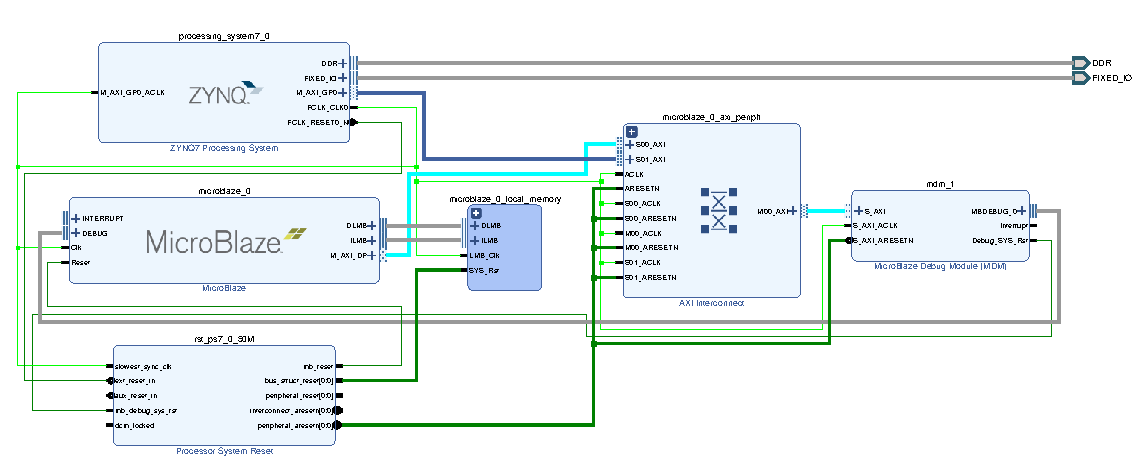
\includegraphics[width=1.0\linewidth]{images/chapter4/mb_base_design_edit.pdf}
\caption{Schematic of a basilar MicroBlaze design}
\label{fig:base_mb}
\end{figure}

In the schematic, the following blocks are present:
\begin{itemize}
    \item \textit{ZYNQ7 Processing System}: it represents the ZYNQ7020's Processing System (PS) from the point of view of the Programmable Logic (PL), as explained in Chapter \ref{sec:pynq}. It can offer a wide range of functionalities to the PL. For the moment, it is only used as a clock source and as a reset source. Via the ZYNQ7 PS block's configuration wizard, it is possible to configure a Phase-Locked Loop (PLL) in order to generate a clock for the PL with a specific frequency. For now, the PLL is configured to generate a clock for the PL with a frequency of 50 MHz, the same as the reference one given by the PYNQ-Z2 board.
    \item \textit{Processor System Reset}: is a soft IP that provides a mechanism to handle the reset conditions for a given system. The core handles numerous reset conditions at the input and generates appropriate resets at the output. For this simple design, the PSR can handle reset requests both from the PS and from the \textit{Debug Core}. It generates an active-high reset signal for the MicroBlaze core and for the Local Memory. Moreover, it generates an acthive-low reset signal for the AXI peripherals. 
    \item  \textit{MicroBlaze}: it represents the MicroBlaze instance under test. It has as inputs some debug signals from the Debug Core, the clock and the reset signal coming from the PSR. It offers as outputs the two memory buses for the Local Memory, one for the data memory (DLMB) and one for the instruction memory (ILMB). The last output is the AXI bus, which is used to access the peripherals through a \textit{AXI Interconnect}.
    \item \textit{Local Memory}: it is a sub-design (automatically generated by Vivado) that interfaces some BRAMs (a special kind of memory offered by the FPGA) with the Local Memory Bus (LMB). Block RAMs (or BRAMs) means Block Random Access Memory. Block RAMs are used for storing large amounts of data inside FPGAs.
    \item \textit{AXI Interconnect}: it is a sub-design (automatically generated by Vivado). As the name suggests, it is used to connect one or more AXI memory-mapped master devices to one or more memory-mapped slave devices.
    \item \textit{MicroBlaze Debug Module}: it is the Debug Core, and its main job is to enable JTAG-based software debugging of the MicroBlaze core. Moreover, it includes a configurable UART via an AXI interface. The UART's \textit{RX} and \textit{TX} signals are transmitted over the device JTAG port and can be accessed via the XSCT tool. With this setup, XSCT offers designers the possibility to interact with the MicroBlaze core via a UART and to control the MicroBlaze core (status, registers, and software debug in general).
\end{itemize}

\begin{figure}[H]
\centering
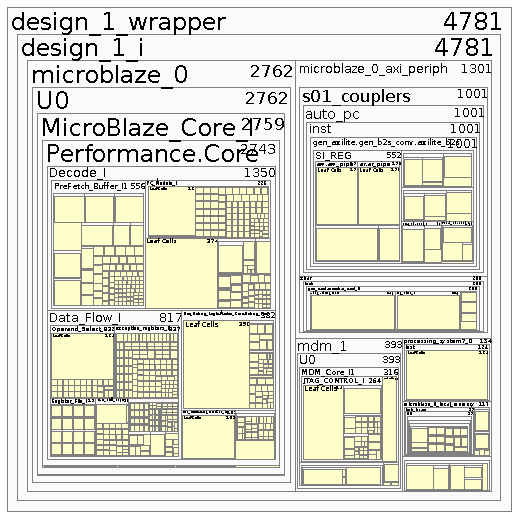
\includegraphics[width=0.6\linewidth]{images/chapter4/hier.png}
\caption{Resulting hierarchy of the MicroBlaze design}
\label{fig:hier_mb}
\end{figure}

By looking at the schematic, there are two AXI masters connected to the AXI Interconnect. Hence, there are two different memory address spaces, and they are configured as follows:\bigskip

\begin{bytefield}{24}
    \begin{rightwordgroup}{/microblaze\_0}
        \memsection{0x4140\_0fff}{0x4140\_0000}{3}{4 KB MDM UART}\\
        \memsection{0x413f\_ffff}{0x0001\_0000}{3}{-- reserved --}\\
        \memsection{0x0000\_ffff}{0x0000\_0000}{6}{64 KB DLMB}
    \end{rightwordgroup}\\\\
    \begin{rightwordgroup}{/processing\_system7\_0}     
        \memsection{0x4140\_0fff}{0x4140\_0000}{3}{4 KB MDM UART}
    \end{rightwordgroup}
\end{bytefield}\bigskip

Finally, the design definition is ready and it can be synthesized and implemented. Because the aim of this design is to be analyzed by injecting faults, the MicroBlaze has been constrained to be placed in a specific portion of the FPGA, as explained in Chapter \ref{sec:fitollo}. This is possible with Vivado by defining a PBLOCK. \bigskip

A PBLOCK is a collection of cells, grouped in one rectangular area or region that specify the device resources contained by the PBLOCK. PBLOCKs are used during floorplanning. A design floorplan is broadly defined as a set of physical constraints used to control how the logic is placed into the FPGA. A good floorplan can help reduce routing congestion and improve the quality of timing results. On the other hand, a bad floorplan can reduce performances as well as unmet constraints if the required placement is unfeasible. \bigskip

As an example, the above design is implemented with the following constraints:\smallskip

\begin{lstlisting}[style=tcl]
create_pblock pblock_1
add_cells_to_pblock [get_pblocks pblock_1] [
    get_cells -quiet [
        list design_1_i/microblaze_0
    ]
]

resize_pblock [get_pblocks pblock_1] -add {
    SLICE_X54Y102:SLICE_X67Y148
}

set_property IS_SOFT 0 [get_pblocks pblock_1]
\end{lstlisting}

In the above constraints, a PBLOCK called \textit{pblock\_1} is first defined. Then all the cells belonging to the Microblaze instance (\textit{design\_1\_i/microblaze\_0}) are added to the PBLOCK, and finally, the PBLOCK is resized. The resize operation is used to define the physical resources that are included in the PBLOCK. As the final operation, the PBLOCK is marked as a \textit{not soft PBLOCK}, which means that each MicroBlaze cell must be placed obligatorily in that specific PBLOCK, and so it is a hard constraint.\bigskip

Once the constraints are ready, the design can be synthesized and implemented. The resulting floorplan is shown in the following figure:

\begin{figure}[H]
\centering
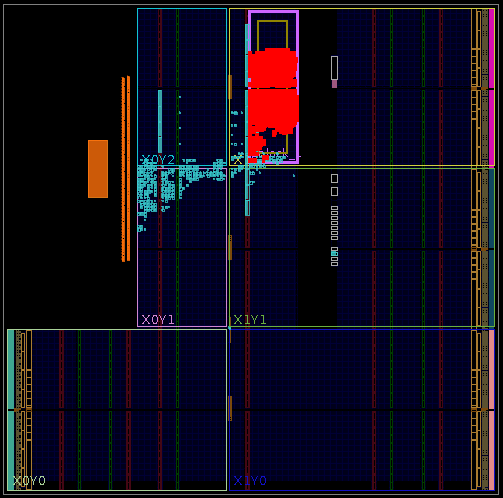
\includegraphics[width=0.8\linewidth]{images/chapter4/impl.png}
\caption{Resulting floorplan of the MicroBlaze design, with the PBLOCK on the top side. Microblaze cells are highlighted in red}
\end{figure}

Finally, it is possible to launch the fault injection tool by providing the bitstream with no CRC and a .elf file to be executed by the MicroBlaze at each run. The resulting fault injection campaign is shown in the following:

\begin{table}[H]
\small
\centering
\begin{tabular}{ l|rr }
    \hline
    \multicolumn{3}{|c|}{\textbf{Functional Analysis}} \\
    \hline
    &\textit{Total}&\textit{Percentage} \\
    \cline{2-3}
    Correct results & 9618 & 77.94 \%\\
    Faulty results (SDE) & 131 & 1.06 \%\\
    MicroBlaze halted & 2359 & 19.12 \%\\
    Raised exceptions & 233 & 1.89 \%\\
    \hline
    Total injected bitflips & 12341 & 100.00 \%\\
    \\
    \hline
    \multicolumn{3}{|c|}{\textbf{Exceptions}}\\
    \hline
    &\textit{Total}&\textit{Percentage} \\
    \cline{2-3}
    \small
    \texttt{XEXC\_ID\_FSL} & 2 & 0.02 \%\\
    \texttt{XEXC\_ID\_UNALIGNED\_ACCESS} & 65 & 0.53 \%\\
    \texttt{XEXC\_ID\_ILLEGAL\_OPCODE}& 107 & 0.87 \%\\
    \texttt{XEXC\_ID\_M\_AXI\_I\_EXCEPTION\_or\_XEXC\_ID\_IPLB\_EXCEPTION} & 0 & 0.0 \%\\
    \texttt{XEXC\_ID\_M\_AXI\_D\_EXCEPTION\_or\_XEXC\_ID\_DPLB\_EXCEPTION} & 55 & 0.45 \%\\
    \texttt{XEXC\_ID\_DIV\_BY\_ZERO} & 3 & 0.02 \%\\
    \texttt{XEXC\_ID\_STACK\_VIOLATION\_or\_XEXC\_ID\_MMU} & 0 & 0.0 \%\\
    \texttt{XEXC\_ID\_FPU} & 0 & 0.0 \%\\
    \hline
\end{tabular}
\caption{Fault injection result for the basic MicroBlaze design}
\label{tab:fi_base}
\end{table}

% \newpage
% \begin{lstlisting}[style=preformatted]
% Total injected bitflips = 12341

%     --- FUNCTIONAL ANALYSIS ---
% Correct results -> 9618 [77.94%]
% Faulty results(SDE) -> 131 [1.06%]
% MicroBlaze halted -> 2359 [19.12%]
% Total exceptions -> 233 [1.89%]

% EXCEPTIONS:


% \end{lstlisting}

% Total injected bitflips = 12555

% Correct results -> 11743 [93.53%]
% Faulty results(SDE) -> 0 [0.0%]
% MicroBlaze halted -> 744 [5.93%]
% Total exceptions -> 68 [0.54%]

% EXCEPTIONS:
%  - XEXC_ID_FSL = 0 [0.0%]
%  - XEXC_ID_UNALIGNED_ACCESS  = 19 [0.15%]
%  - XEXC_ID_ILLEGAL_OPCODE  = 36 [0.29%]
%  - XEXC_ID_M_AXI_I_EXCEPTION_or_XEXC_ID_IPLB_EXCEPTION = 0 [0.0%]
%  - XEXC_ID_M_AXI_D_EXCEPTION_or_XEXC_ID_DPLB_EXCEPTION = 13 [0.1%]
%  - XEXC_ID_DIV_BY_ZERO  = 0 [0.0%]
%  - XEXC_ID_STACK_VIOLATION_or_XEXC_ID_MMU  = 0 [0.0%]
%  - XEXC_ID_FPU  = 0 [0.0%]

From the above results, it is possible to see that in the majority of the cases, the MicroBlaze correctly executes its job. This is because the executed firmware possibly stimulates only a sub-part of the core. However, there are a lot of faulty cases ($> 21\%$), and they are divided into three categories:

\begin{itemize}
    \item \textit{SDE}: the MicroBlaze executes the entire code until the end (the end condition is detected when the MicroBlaze prints a specific string, like \texttt{DONE\_1 DONE\_1 DONE\_1}). However, the output differs in some measures from the golden one.
    \item \textit{Halted}: the MicroBlaze is halted, meaning that the end condition is not detected.
    \item \textit{Exception}: the MicroBlaze raised an exception.
\end{itemize}

Even tho SDEs and exceptions can be directly detected by the firmware running on the core, it is not possible to detect the halted state. In theory, would be possible to detect and try to correct the FPGA configuration. Nonetheless, trying to do so would lead to two main problems:

\begin{enumerate}
    \item Halt conditions are the majority of the cases ($> 19\%$ or about $86\%$ among the faulty conditions). In this case, the firmware is almost not able to run and the fault would not be detected.
    \item During SDEs or exceptions, the MicroBlaze runs until the end of the code, but it is not guaranteed that all the instructions are executed or are executed correctly. 
\end{enumerate}

Thus, a different approach is needed to detect and correct the fault.

% Explain here what are the effects of SEUs in the MicroBlaze.

\section{Strategies and adopted solutions}

Because of the problems raised in the previous section, different approaches need to be evaluated. This thesis work is focused on SEUs affecting the configuration layer of the FPGA, as they are more likely to occur. The adopted strategy can detect and correct those errors, previously defined as persistent errors, and may correct errors in the application layer too, under the condition that the overall design (hardware or software) is engineered in such a way to detect them. \bigskip

To overcome those persistent errors, there are some techniques able to exploit the particular reconfigurable capabilities of the FPGAs. The following are some of the techniques taken into account:

\begin{description}
    \item[Data Scrubbing] is a general technique based on the concept of a virtual background task that periodically checks memory content for errors, then corrects detected errors using redundant data in the form of different checksums or copies of data. It is useful to correct and prevent (accumulation) errors in the information stored in memory. In FPGAs, scrubbing can be used to mitigate both persistent errors in SRAM cells (i.e., the configuration memory) and transient errors in user-memory elements such as BRAMs. To perform configuration memory scrubbing, the configuration memory data must be read sequentially from the start to the end and compared to the original configuration bitstream or an error check code such as a cyclic redundancy check (CRC). Scrubbing can be performed (both check and correction) without interrupting the device's functionalities. In aerospace applications, scrubbing is a common technique to mitigate the effects of SEUs. However, there are a few aspects to overcome like often the scrub operation must be performed, because of the very limited area and power constraints. Hence, scrubbing alone is a weak mitigation strategy without any other technique applied \cite{nasa_scrubbing}. This is mainly because if a configuration bit is hit while the circuit is active, the error propagates in the design and can lead to a failure and the scrubber has no time to fix the error. An example of good design would be having a scrubber joined by a design with a triple modular redundancy check. The TMR design can detect and mask the error by itself, without causing a failure and meanwhile, the scrubber can be notified of the error and fix it. In this sense, scrubbing can be useful against error accumulation too.
    \item[Dynamic partial reconfiguration] \cite{10.1007/978-3-030-44534-8_7} allows run-time reconfiguration without application layer interruption. This technique cannot detect errors by itself, so it must be combined with other error detection techniques such as those based on redundancy. These correction techniques take advantage of the subdivision of the configuration memory into frames, which contain information related to the configuration of specific parts of the design. While these techniques allow increasing the protection capability against radiation effects, they introduce several penalties to the design, particularly in terms of performance. In literature, some techniques are proposed, like innovative placement algorithms able to improve the running frequency up to 44\% by reducing the interconnection delays between resources \cite{10.1145/1366224.1366228}.
\end{description}

The chosen strategy is to use the Dynamic Partial Reconfiguration technique. For this thesis work, only the MicroBlaze area is configured as dynamic reconfigurable. As said, this is useful only to fix errors in the configuration area related to the FPGA, but something that detects the error is needed. Hence, a self-made watchdog is developed to detect the error and trigger the reconfiguration. The reconfiguration is handled by a dedicated controller. A high-level scheme of the design is presented in the following figure:
% Watchdog + DFX because..

\begin{figure}[H]
\centering
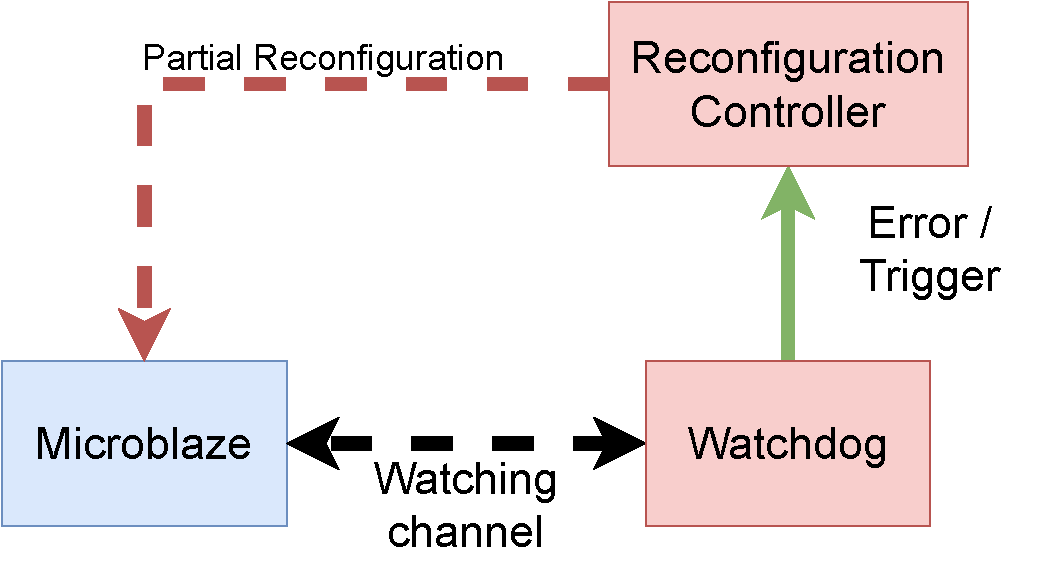
\includegraphics[width=0.8\linewidth]{images/chapter4/reconf_scheme.pdf}
\caption{High level scheme of the fault tolerant design.}
\label{fig:reconf_scheme}
\end{figure}

In figure \ref{fig:reconf_scheme}, the following parts are highlighted:
\begin{description}
    \item[MicroBlaze] it is intended both as the instance of the MicroBlaze itself and as the physical area of the FPGA where the MicroBlaze is mapped and configured as dynamic reconfigurable.
    \item[Watchdog] its job is to continuously check the MicroBlaze's status via a \textit{watching channel} (that is, a channel that is used to monitor the MicroBlaze's status) and if the MicroBlaze is halted, it triggers the reconfiguration via a dedicated signal \textit{Error/Trigger}.
    \item[Reconfiguration Controller] it is the controller that handles the partial reconfiguration when it is signaled to do so by the watchdog. It is responsible for the reconfiguration of the MicroBlaze's area.
\end{description}

\section{Development of a watchdog}

Among the modules to be added to the design in order to achieve a fault-tolerant design, the watchdog is the most critical one. If it fails in detecting errors, the overall design doesn't result protected from SEUs affecting the MicroBlaze. This is because the watchdog would not able to detect the error and trigger the reconfiguration. 

\subsection{What is a watchdog?}

In computer systems, a watchdog is essentially a timer (that may be hardware or software) that is used to detect and recover from computer malfunctions. Watchdog timers are widely used in computers to facilitate the automatic correction of temporary hardware faults. Can be thought of as a down-count timer. When the timer elapses, it generates a timeout signal.\bigskip

During normal operation, the computer regularly restarts the watchdog timer to prevent it from timing out. If due to a hardware fault or program error, the computer fails to restart the watchdog, the timer will elapse generating a timeout signal. The timeout signal is used to initiate corrective actions. The act of restarting the watchdog timer is usually called \textit{kicking}. \bigskip

Both generally speaking or strictly related to this case of study, a watchdog timer provides automatic detection of catastrophic malfunctions that prevent the computer from kicking it. However, there are often less severe types of faults that do not interfere with the kicking operation but still require watchdog oversight. In the specific case, can be for example a fault affecting the Arithmetic Logic Unit (ALU) of the MicroBlaze or the AXI interface towards peripherals. To support these, the system should be designed so that the watchdog timer is not kicked anymore in these less-severe faults. This can be done by writing some software routines that can self-test the CPU and its functionalities. The CPU will kick the watchdog only if all tests have passed.

% TODO: add wdctl linux output taken from a raspberry pi

\subsection{How to implement a watchdog?}
\label{sec:wd_impl}

Once understood the principles of a watchdog, it is possible to implement it and tailor its functionalities to the needs of having a fault-tolerant system on FPGA. From a high-level perspective, the watchdog is at heart a timer. This means that it must have some form of timing, so it needs a clock and reset signals. Moreover, the timer must restart every time the kicking action is performed. If the timer elapses, it generates a timeout signal. The following is a timing diagram of this basic watchdog:

\begin{figure}[H]
\begin{tikztimingtable}[%
    timing/dslope=0.10,
    timing/.style={x=5ex,y=2ex},
    x=5ex,
    timing/rowdist=3ex,
    timing/name/.style={font=\sffamily\scriptsize}
]
\busref{CLK}          & 25{c} \\
\busref{RST}          & 1L H 10Ll \\
\busref[1::0]{COUNT}  & Uu 1D{$3$} 1D{$2$} D{$1$} D{$3$} D{$2$} D{$2$} D{$1$} 4D{$0$} \\
\busref{KICK}         & 1U 3L H 7Ll \\
\busref{TIMEOUT}      & 1Uu 3L 5L 3H \\
\extracode
\begin{pgfonlayer}{background}
\begin{scope}[semitransparent ,semithick]
\vertlines[darkgray,dotted]{0.5,1.5 ,...,11.5}
\vertlines[green,dashed,opacity=1]{4.5}
\vertlines[red,dashed,opacity=1]{9.5}
\end{scope}
\end{pgfonlayer}
\end{tikztimingtable}
\caption{Timing diagram of a very basic watchdog.}
\label{fig:basic_watchdog}
\end{figure}

In figure \ref{fig:basic_watchdog}, the system initially is in an unknown state. Once the reset signal \textit{RST} arrives, synchronously the watchdog is reset and starts counting down. When the timer reaches 1, luckily a \textit{KICK} signal arrives (green line), signaling that the CPU is correctly working, and the timer is restarted from the initial value of 3. 4 clock cycles later, the timer reaches 0, and the \textit{TIMEOUT} signal is generated (red line) because no \textit{KICK} signal has arrived. \bigskip

A more sophisticated implementation of a watchdog could be based on a up-count timer, an input data containing the maximum number of clock cycles the timer can count before it generates a timeout signal, and a start signal that is used to start the timer. The following is a timing diagram of this implementation:

\begin{figure}[H]
\begin{tikztimingtable}[%
    timing/dslope=0.10,
    timing/.style={x=5ex,y=2ex},
    x=5ex,
    timing/rowdist=3ex,
    timing/name/.style={font=\sffamily\scriptsize}
]
\busref{CLK}          & 25{c} \\
\busref{RST}          & 1L H 10Ll \\
\busref[2::0]{VALUE}  & U 3D{$7$} 17d{$3$}\\
\busref{START}        & U L H 9Ll\\\\
\busref[2::0]{COUNT}  & Uu 2D{$0$} 1D{$1$} D{$0$} D{$1$} D{$2$} D{$0$} D{$1$} D{$2$} 2D{$3$} \\
\busref{KICK}         & 1U 3L H 2L H 4Ll \\
\busref{TIMEOUT}      & 1Uu 3L 7L H \\
\extracode
\begin{pgfonlayer}{background}
\begin{scope}[semitransparent ,semithick]
\vertlines[darkgray,dotted]{0.5,1.5 ,...,11.5}
\vertlines[NavyBlue,dashed,opacity=0.9]{2.5}
\vertlines[green,dashed,opacity=1]{4.5, 7.5}
\vertlines[red,dashed,opacity=1]{11.5}
\end{scope}
\end{pgfonlayer}
\end{tikztimingtable}
\caption{Timing diagram of a more sophisticated watchdog.}
\label{fig:basic_watchdog_upcount}
\end{figure}

In the figure above, we have a different working mechanism compared to the previous one. After the reset signal \textit{RST}, the timer is reset to its initial value of 0 and stays in this state until the \textit{START} signal is received. At this point, the input value \textit{VALUE} is set at 7 from the external: 7 is the final value of the timer, if this value is reached, the timer expires. Once the \textit{START} signal is received (blue line), the timer starts counting up. The next clock cycle sees a change in the maximum value, from 7 down to 3. The \textit{KICK} signal is generated two times (green line), signaling that the CPU is correctly working, and the timer is restarted from 0. At a certain point in time, the timer reaches 3 but the \textit{KICK} signal is not arriving, thus at the next clock cycle the \textit{TIMEOUT} signal is generated (red line).

\begin{figure}[H]
\centering
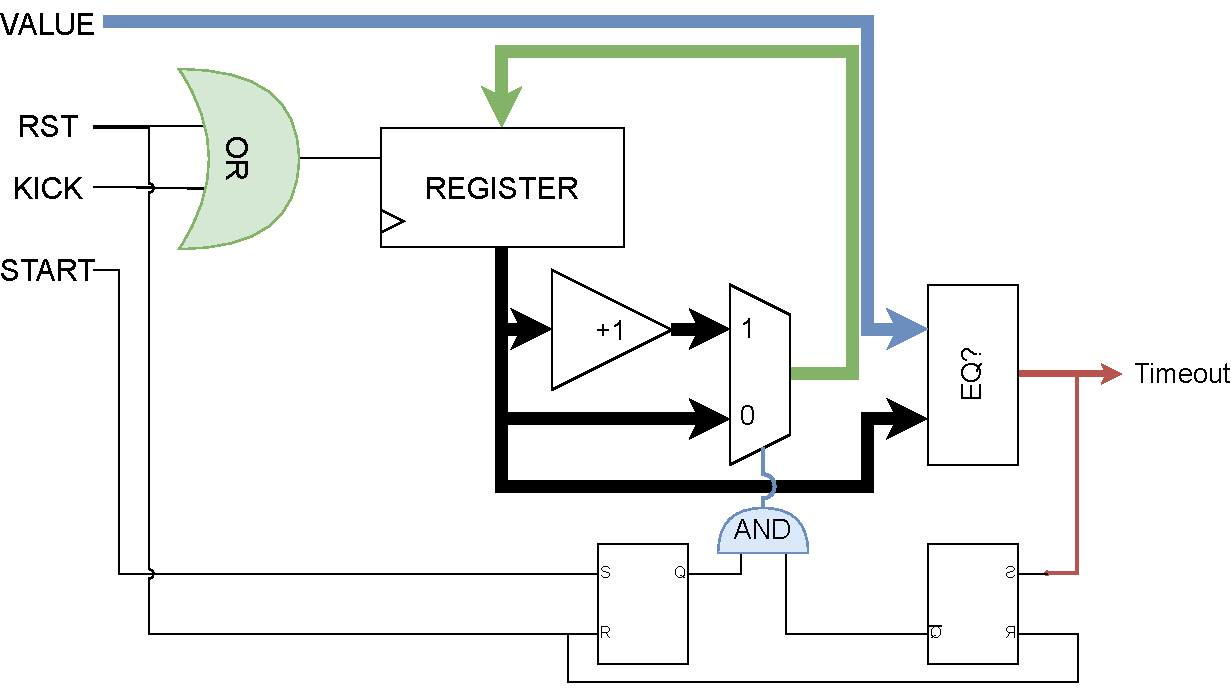
\includegraphics[width=0.8\linewidth]{images/chapter4/impl_schem_wd.pdf}
\caption{Possible digital circuit implementation of a watchdog.}
\label{fig:wd_scheme}
\end{figure}

This implementation can be used as it is and can achieve good results. A possible circuit implementation, even with some timing differences, can be seen in Figure \ref{fig:wd_scheme}. The problem is that the \textit{KICK} signal represents a single point of failure in terms of fault tolerance. If the CPU is hit by an SEU, it can leave the signal stuck in a high state, and the watchdog will continuously reset the timer, maskin the real CPU's status. \bigskip

To overcome this problem, a more sophisticated signaling mechanism is used. To keep things simple, the act of kicking is done at every $H\rightarrow L$ or $L\rightarrow H$ transition of the \textit{KICK} signal. This way, if the signal is stuck in a certain state, the watchdog will expire correctly. The final circuit implementation is based on a Finite State Machine, that is, a set of states that are interconnected by transitions. It is faster to implement when things get more complicated, and it is easier to understand than the previous diagram. The following is a diagram of the Finite State Machine that implements the final version of the watchdog:

\begin{tikzpicture} [draw=cyan!70!black,
    node distance = 2.5cm, 
    on grid, 
    auto,
    every loop/.style={stealth-},
    every initial by arrow/.style={darkgreen}]

% Help grid
% \draw [help lines] (-7,5) grid (7,-5);
% \node (ref) [state] at (0,0) {};

% State S_START
\node (qs) [state with output,
    darkgreen,
    text = black,
    initial left,
    initial text = {$RST$}] at (-4, -4) {START \nodepart{lower} $count = 0$};
 
% state DOOMED
\node (qd) [state with output, red, text = black, accepting] at (4, 4) {DOOMED \nodepart{lower} $timeout = 1$};

% State q0 
\node (q0) [state with output] at (-3, 3) {CHECK 0 \nodepart{lower} $count \mathrel{+{=}} 1$};
 
% State q1    
\node (q1) [state with output] at (3, -3) {CHECK 1 \nodepart{lower} $count \mathrel{+{=}} 1$};
 
% Arrows
\path [-stealth, thick]
    (qs) edge [darkgreen, bend left] node[black, pos = 0.2, align=center] {$start = 1$\\$kick = 1$} (q0)
    (qs) edge [darkgreen, bend right] node[below, pos = 0.2, black, align=center] {$start = 1$\\$kick = 0$} (q1)
    (q0) edge [red, bend left] node[black, pos=0.6, align=center] {$count \geq value$\\$kick=1$} (qd)
    (q1) edge [red, bend right] node[black, pos = 0.2, right, align=center] {$count \geq value$\\$kick=0$} (qd)
    (q0) edge[bend left] node[align=center] {$count \leq value$\\$kick = 0$}   (q1)
    (q1) edge[bend left] node[align=center] {$count \leq value$\\$kick = 1$}   (q0)
    (q0) edge [loop above]  node[align=center] {$count < value$\\$kick = 1$}()
    (q1) edge [loop below]  node[align=center] {$count < value$\\$kick = 0$}()
    (qd) edge [red, in=30,out=60, loop] node {} ();
\end{tikzpicture}

Formally speaking, this FSM is a Moore machine. In the theory of computation, it means that the current output values are determined only by the FSM current state \cite{Church1958EdwardFM}. Inputs only affect the next state, and state transitions may happen only at each rising edge of the clock signal. \bigskip

The idea behind the logic of this FSM is that at the reset, the FSM waits for the START signal. Once it is detected, it goes into a loop between two complementary states. They are implemented in such a way to be able to detect signal transitions. The FSM stays in this loop until the count reaches the input value, and if this happens and the kick signal still doesn't toggle, the FSM goes into a final state asserting the timeout signal. The FSM will stay in this state until it is reset again. If the input timeout value changes, it is captured only when a transition is detected. The following is a description of the states in the FSM:

\begin{table}[H]
\centering
\begin{tabular}{ l|c|p{9.5 cm} }
    State&Output&Brief Description\\
    \cline{1-3}
    \multirow{7}{*}{\texttt{START}} & \multirow{7}{*}{\begin{tabular}{@{}r@{}}\texttt{COUNT = 0}\\\texttt{TIMEOUT = 0}\\\texttt{STARTED = 0}\end{tabular}} & This is the initial state after the reset of the machine. Here the count stays at 0, waiting for start = 1. When the start signal is asserted, it goes to CHECK 1 or CHECK 0, depending on the current kick value (because of the transition detection, if kick = 0, the watchdog waits for kick = 1, $L\rightarrow H$ transition, and vice versa).\\
    \hline
    \multirow{6}{*}{\texttt{CHECK 0}} & \multirow{12}{*}{\begin{tabular}{@{}r@{}}\texttt{COUNT += 1}\\\texttt{TIMEOUT = 0}\\\texttt{STARTED = 1}\end{tabular}} & Watchdog started and waiting for the kick signal to go low. When the kick signal goes low, the FSM goes to CHECK 1, detecting the $H\rightarrow L$ transition. While the transition is not detected, the count keeps increasing at each clock tick. When the count reaches the input value, the watchdog goes to DOOMED.\\
    \cline{1-1}
    \cline{3-3}
    \multirow{6}{*}{\texttt{CHECK 1}} && Watchdog started and waiting for the kick signal to go high. When the kick signal goes high, the FSM goes to CHECK 0, detecting the $L\rightarrow H$ transition. While the transition is not detected, the count keeps increasing at each clock tick. When the count reaches the input value, the watchdog goes to DOOMED.\\
    \hline
    \multirow{3}{*}{\texttt{DOOMED}} & \multirow{3}{*}{\begin{tabular}{@{}r@{}}\texttt{COUNT += 0}\\\texttt{TIMEOUT = 1}\\\texttt{STARTED = 1}\end{tabular}} & The watchdog is expired. The timeout signal is asserted and the FSM waits indefinitely until a reset arrives.\\
    \hline
\end{tabular}
\caption{Detailed explanation of the states of the FSM}
\end{table}

\begin{figure}[H]
\begin{tikztimingtable}[%
    timing/dslope=0.10,
    timing/.style={x=5ex,y=2ex},
    x=5ex,
    timing/rowdist=3ex,
    timing/name/.style={font=\sffamily\scriptsize}
]
\busref{CLK}          & 25{c} \\
\busref{RST}          & 1L H 10Ll \\
\busref[2::0]{VALUE}  & U 3D{$7$} 17d{$2$}\\
\busref{START}        & U L H 9Ll\\
\busref{KICK}         & 1U 3L 3H 2L L 2Ll \\
\\
\busref{STATE}  & Uu 1D{$START$} 2D{$CHECK 1$} 6D{$CHECK 0$} 2D{$DOOMED$}\\
\busref[2::0]{COUNT}  & Uu 2D{$0$} 1D{$1$} D{$0$} D{$1$} D{$2$} D{$0$} D{$1$} 3D{$2$} \\
\busref{TIMEOUT}      & 1Uu 3L 6L 2H \\
\busref{STARTED}      & 1Uu 1L 6H 4H \\
\extracode
\begin{pgfonlayer}{background}
\begin{scope}[semitransparent ,semithick]
\vertlines[darkgray,dotted]{0.5,1.5 ,...,11.5}
\vertlines[NavyBlue,dashed,opacity=0.9]{2.5}
\vertlines[green,dashed,opacity=1]{4.5, 7.5}
\vertlines[red,dashed,opacity=1]{10.5}
\end{scope}
\end{pgfonlayer}
\end{tikztimingtable}
\caption{Timing diagram of a more sophisticated watchdog.}
\label{fig:final_wd_wafe}
\end{figure}

The FSM has been implemented as a High-Level State Machine (HLSM). An HLSM is a natural extension of an FSM, used to capture more complex behaviors, including multi-bit data inputs and outputs rather than just single bits, local storage and supports arithmetic operations like adds and comparisons, rather than just basic boolean operations. It has been implemented in VHDL and the code is available in Appendix \ref{sec:watchdog_fsm}. In figure \ref{fig:final_wd_wafe}, the timing diagram of the final watchdog behavior is presented.

\subsection{How to harden the watchdog?}

Once the watchdog is implemented, it needs to be hardened. This is needed to prevent the watchdog from being inhibited by an SEU affecting it. The most basic type of fault tolerance technique is the Triple Modular Redundacy (TMR). It basically consists in having three different modules that, given the same input generate the same output in normal conditions. The three outputs are given as input to a voter circuit.

\begin{figure}[H]
\centering
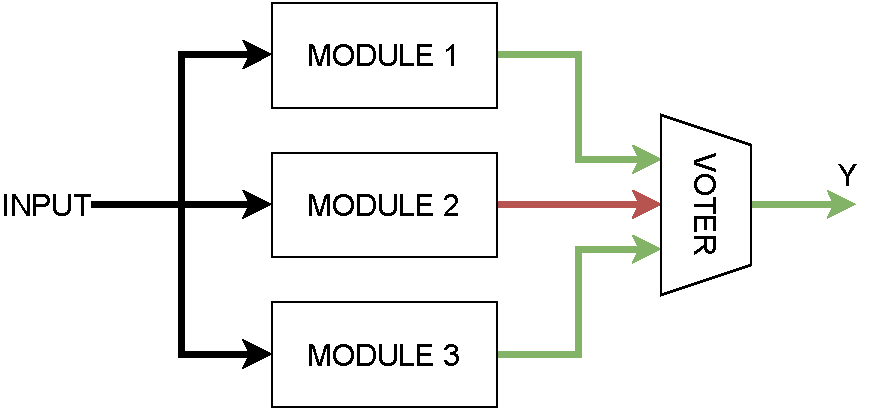
\includegraphics[width=0.9\linewidth]{images/chapter4/tmr.pdf}
\caption{Triple Modular Redundacy (TMR) scheme.}
\label{fig:tmr_scheme}
\end{figure}

The three modules can be identical or have a different implementation, but they must all generate the same output given the same input. \bigskip

The voter circuit is a majority-voting system, which means that if all the three outputs are the same, the voter circuit gives as output one of the three inputs. If one of the three outputs is different (because one of the three modules is faulty), the voter circuit is capable of detecting the difference and outputs the non-faulty result. Thus, the fault is masked and it is not propagated to the rest of the system. The truth table of a 1-bit voter circuit is the following:

\begin{table}[H]
\centering
\begin{tabular}{ ccc|c }
    \textbf{A}&\textbf{B}&\textbf{C}&\textbf{Y}\\
    \hline
    0&0&0&0\\
    0&0&\textcolor{red}1&0\\
    0&\textcolor{red}1&0&0\\
    \textcolor{red}0&1&1&1\\
    \textcolor{red}1&0&0&0\\
    1&\textcolor{red}0&1&1\\
    1&1&\textcolor{red}0&1\\
    1&1&1&1\\
\end{tabular}
\caption{Voter truth table. The red cells indicate the faulty output.}
\end{table}

It can be implemented as a circuit in the following way:
\begin{equation}
\begin{aligned}
Y ={} & \text{majority}(A, B, C) = AB + AC + BC = \\
      & \overline{\overline{AB}} + \overline{\overline{AC}} + \overline{\overline{BC}} = \overline{\overline{AB}\cdot\overline{AC}\cdot\overline{BC}}
\end{aligned}
\end{equation}

\begin{figure}[H]
\centering
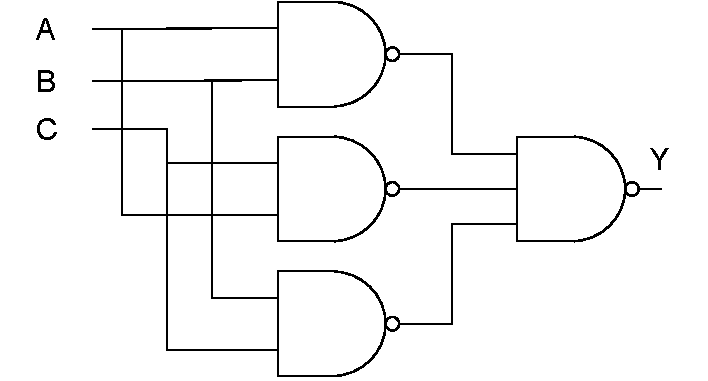
\includegraphics[width=0.7\linewidth]{images/chapter4/tmr_circuit.pdf}
\caption{1-bit voter circuit scheme.}
\label{fig:voter_scheme}
\end{figure}

The majority gate itself could fail, representing a single point of failure. This can be protected by applying triple redundancy to the voters themselves. Hence, three voters are used, one for each copy of the next stage of TMR logic, as shown in the following figure:

\begin{figure}[H]
\centering
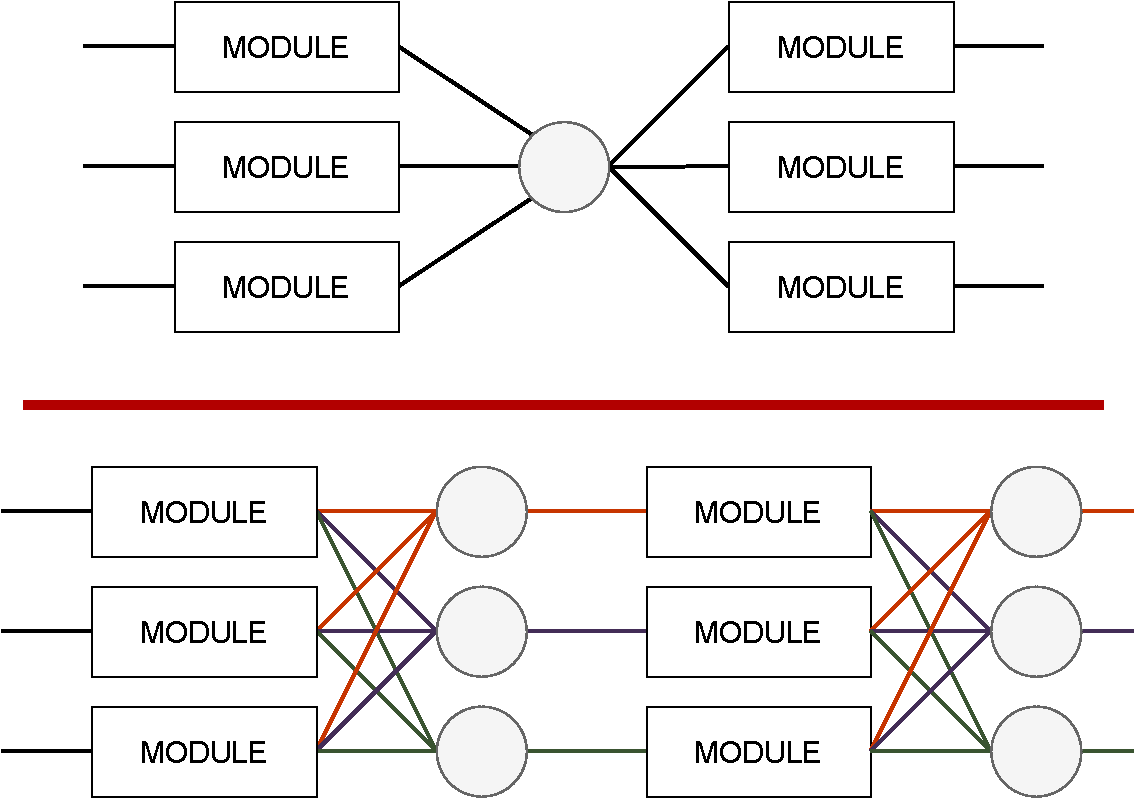
\includegraphics[width=0.9\linewidth]{images/chapter4/tmr_voter.pdf}
\caption{Basic TMR scheme vs. full TMR circuit scheme.}
\end{figure}

Even tho the second scheme doesn't present any single point of failure, most systems stick with the simplest scheme. This is because the majority of gates are much less complex than the systems that they guard against, so they are much more reliable. In those cases, by using some reliability calculations, it is possible to find the minimum voter realiability required to have a fully functional TMR scheme. \bigskip

However, because this section is about how to harden a watchdog implemented in FPGA, even interconnections can be affected by faults due to SEUs affecting the route part of the configuration layer. Consequently, a full TMR scheme is the most reliable way to protect the watchdog.\bigskip

Hence, the idea is to instantiate the watchdog component three different times and vote each input and output with three different voters. The overall design is implemented in Verilog. To simplify the code, two matrices of signals have been created: one for the no-tmr version and one for the tmr version. As an example, because of the full TMR scheme, there are three different \textit{START} signals (at this point of the design, the driver of these signals is not yet specified). The idea is to access these 3 different instantiations of signals by using indexes and not directly the signals themselves with different names (for example \textit{START_0}, \textit{START_1} and \textit{START_2}) to not create a confusional code and to be able to automatize the code generation.

\begin{figure}[H]
\centering
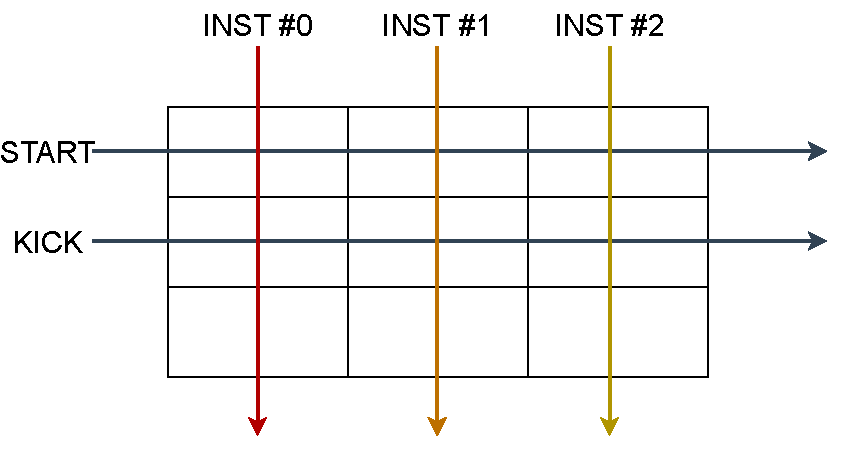
\includegraphics[width=0.8\linewidth]{images/chapter4/mtx_notmr.pdf}
\caption{Input signal matrix for the no-tmr version.}
\label{fig:mtx_notmr}
\end{figure}

The above scheme can be read as follows:
\begin{itemize}
    \item The START (KICK) signal instance 0 is at row 0 (1), column 0.
    \item The START (KICK) signal instance 1 is at row 0 (1), column 1.
    \item The START (KICK) signal instance 2 is at row 0 (1), column 2.
\end{itemize}

The same concept applies to the output signals of the voters. Three voters create three different output signals and each voter has as input the same triplet of signals as the other ones. Hence, the tmr matrix works as the no-tmr one. The following table shows an example, supposing the no-tmr matrix is configured as the one shown in Figure \ref{fig:mtx_notmr} for what concerns the \textit{START} signal:

\begin{table}[H]
\centering
\begin{tabular}{ r|ccc|c }
    \textbf{Voter \texttt{\#}}&\textbf{A}&\textbf{B}&\textbf{C}&\textbf{Y}\\
    \hline
    1 & \texttt{NOTMR[0][0]} & \texttt{NOTMR[0][1]} & \texttt{NOTMR[0][2]} & \texttt{TMR[0][0]}\\
    2 & \texttt{NOTMR[0][0]} & \texttt{NOTMR[0][1]} & \texttt{NOTMR[0][2]} & \texttt{TMR[0][1]}\\
    3 & \texttt{NOTMR[0][0]} & \texttt{NOTMR[0][1]} & \texttt{NOTMR[0][2]} & \texttt{TMR[0][2]}\\
\end{tabular}
\caption{Output signal matrix for the no-tmr version.}
\end{table}

The main problem with this solution is that all the three voters are doing exactly the same things on the same inputs and producing the same outputs. Ideally, this is the aim of the design, but once it is synthesized, everything is collapsed into a single voter and a single watchdog. This happens because the synthesizer tries to optimize the design by reusing and sharing the logic between similar components. A situation that must absolutely be avoided, because the aim is exactly to have three different copies of everything: signals, voters and watchdogs.\bigskip

To overcome this problem, the synthesizer must be notified about what it can optimize and what it can not. The following is an example of instantiation of the two matrices of signals and voters in Verilog, telling the synthesizer that they must not be optimized out:

\begin{lstlisting}[style=Verilog]
(* dont_touch = "true" *) wire notmr[3:0][2:0];
(* dont_touch = "true" *) wire tmr[3:0][2:0];

generate
  genvar jdx;
  for (jdx = 0; jdx < 3; jdx = jdx + 1) begin
      for (idx = 0; idx < 4; idx = idx + 1) begin
          (* dont_touch = "true" *) voter_bus #(
              .NBITS(1)
          ) voter_ith (
              .DATA_IN0(notmr[idx][0]),
              .DATA_IN1(notmr[idx][1]),
              .DATA_IN2(notmr[idx][2]),
              .DATA_OUT(tmr[idx][jdx])
          );
      end
  end
endgenerate
\end{lstlisting}

Finally, the design is implemented. All the inputs that go to the watchdog are taken from the tmr matrix, and all the outputs generated by the watchdogs (for example the three timeout signals) go to the no-tmr matrix. The latter are automatically voted because of the previous instantiation of the voter components, as shown above. The final outputs of the overall TMR Watchdog are connected to the respective TMR version of the signals.

\begin{figure}[H]
\centering
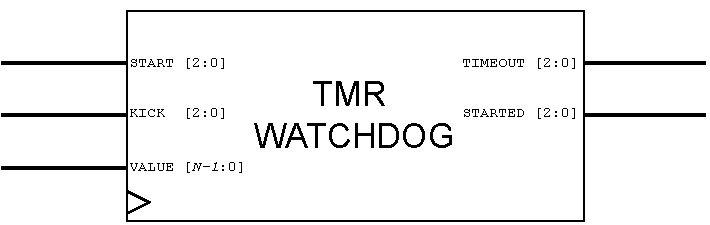
\includegraphics[width=0.7\linewidth]{images/chapter4/wd_tmr.pdf}
\caption{Interfaces of the TMR Watchdog.}
\label{fig:wd_tmr}
\end{figure}

% Insert more complex voter at the end: https://arxiv.org/abs/1605.03771
% ...
% What is a voter?
% Idea behind TMR and voter (doesn't prevent by fault accumulation, but will be explained in the conclusions)
% Paradox: who votes the voter?

\subsection{Integration of the watchdog in the design}

The watchdog is finally created but it is still not easily usable. The goal is to have a watchdog that can be easily inserted into any design. To achieve this, the watchdog can be packaged as an IP to allow the user to easily integrate it with the Block Design tool. Vivado offers an easy-to-use IP creation wizard, through which a design can be packed and distributed, together with a C library for high-level interaction with the hardware via software drivers.\bigskip

Unfortunately, this is not enough. The idea is to connect the watchdog to the MicroBlaze, in this way it would be able to control it (for example the kicking action) and check its status. The problem is that the watchdog uses discrete signals as an interface and there is no direct way to access these signals from the CPU. There are two possible ways to overcome this situation:

\begin{itemize}
    \item The MicroBlaze controls the watchdog via a GPIO peripheral. This is the most simple way to do it, but it is not very flexible. The various GPIO channels are connected to the watchdog signals and the CPU can control the GPIO channels via the AXI interface.
    \item The MicroBlaze direct interfaces with the watchdog through a dedicated AXI interface. This is the most flexible way to do it but increases the implementation complexity of the watchdog IP.
\end{itemize}

% For what concerns this thesis work, 
The second option is the most convenient because there are fewer actors in the overall fault-tolerance chain that can be affected by faults. Luckily, the Vivado IP creation wizard provides an automatic way to create an AXI wrapper on top of which the watchdog can be instantiated and the different signals connected to the various registers. Hence, the watchdog can be controlled and monitored by the MicroBlaze via those, as shown in the following. \bigskip

\begin{figure}[H]
\centering
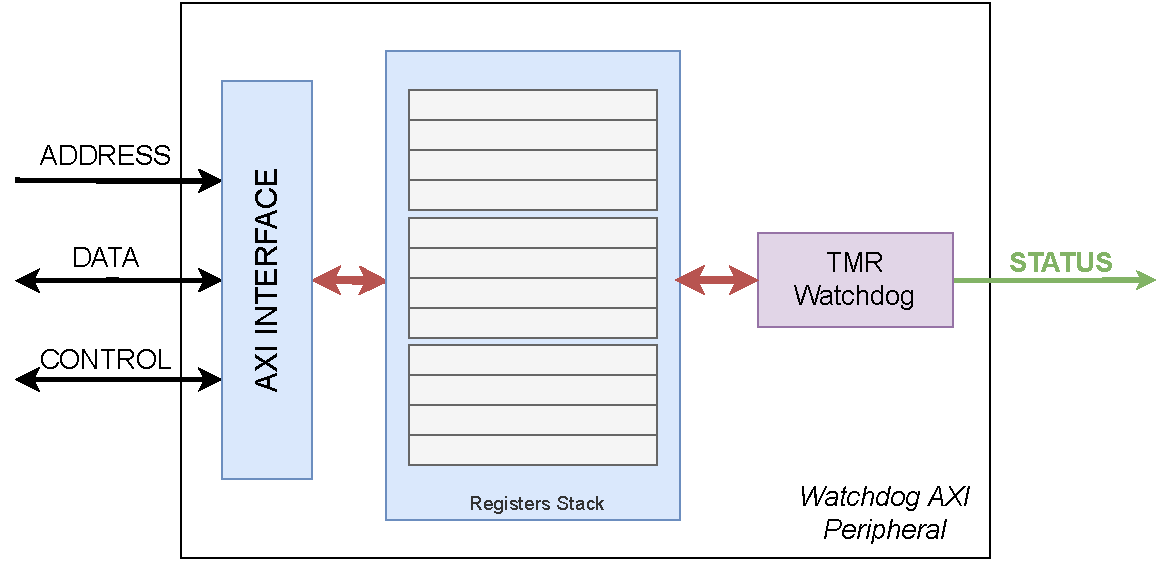
\includegraphics[width=0.75\linewidth]{images/chapter4/rs2.pdf}
\caption{Conceptual representation of the final watchdog IP.}
\label{fig:rs2}
\end{figure}

By design choice, there are 4 registers, one for each of the 3 watchdog instances. The second nibble in the lowest byte of the address is the index of the corresponding watchdog. They follow the Full TMR design as explained in the previous section, internally coded with no-tmr and tmr matrices. Read-only fields are taken from the no-tmr matrix, in this way the CPU or any other AXI master can check if there are faulty modules. \bigskip

The following is a description of how the register space is divided and seen by AXI masters:

\begin{center}
\begin{register}{H}{Control Register}{0x00 - 0x10 - 0x20}% name=example
\regfieldb{}{30}{2}% READ_ONLY
\regfieldb{Kick}{1}{1}%
\regfieldb{Start}{1}{0}%
\begin{regdesc}\begin{reglist}[Request~Depth]
\item [Start]Setting this bit activates the Watchdog. If already activated, this bit has no effects.
\item [Kick]The kick bit is directly connected to the kick signal of the watchdog. The MicroBlaze is in charge of writing the right value in this field (i.e. do the right transitions).
\end{reglist}\end{regdesc}
\end{register}
\begin{register}{H}{Status Register}{0x04 - 0x14 - 0x24}% name=example
\regfieldb{}{30}{2}% READ_ONLY
\regfieldb{Error}{1}{1}%
\regfieldb{Started}{1}{0}%
\begin{regdesc}\begin{reglist}[Request~Depth]
\item [Started]The bit is set if the watchdog is started.
\item [Error]The bit is set if the watchdog timed out.
\end{reglist}\end{regdesc}
\end{register}
\begin{register}{H}{Timeout Register}{0x08 - 0x18 - 0x28}% name=example
\regfieldb{Timeout}{32}{0}% READ_ONLY
\begin{regdesc}\begin{reglist}[Request~Depth]
\item [Timeout]32 bit value that represents the number of cycles required before the watchdog times out.
\end{reglist}\end{regdesc}\
\end{register}
\begin{register}{H}{Toggle Rate Register}{0x0C - 0x1C - 0x2C}% name=example
\regfieldb{Toggle Rate}{32}{0}% READ_ONLY
\begin{regdesc}\begin{reglist}[Request~Depth]
\item [Toggle Rate]32 bit value that represents the actual toggling rate of the watchdog, in clock cycles. The CPU can use it to estimate, for example, if there are differences between the expected toggling rate and the real one.
\end{reglist}\end{regdesc}\
\end{register}
\end{center}

To ease the job of programmers, the Watchdog IP offers a driver with a set of functions to control the watchdog. It is based on a newly defined data type that represents the Watchdog register memory space conveniently, by using C structs, unions and bitfields constructs. The full description is shown in Appendix \ref{sec:watchdog_drivers}.

\begin{lstlisting}[style=C]
typedef struct {
	union {
		u32 *baseAddress;
		watchdog_module_t *module;
		struct {
			watchdog_module_t module0;
			watchdog_module_t module1;
			watchdog_module_t module2;
		} *modules;
	};
} GBcnCtrl;
\end{lstlisting}

Once the Watchdog IP repository han been added to the list of IP repositories in Vivado ($Vivado \rightarrow IP \rightarrow Repository \rightarrow +$), it can be instantiated in the design and connected to a AXI Interconnect to make it accessible to masters, like the MicroBlaze, via an intermediate AXI Interconnect:

\begin{figure}[H]
\centering
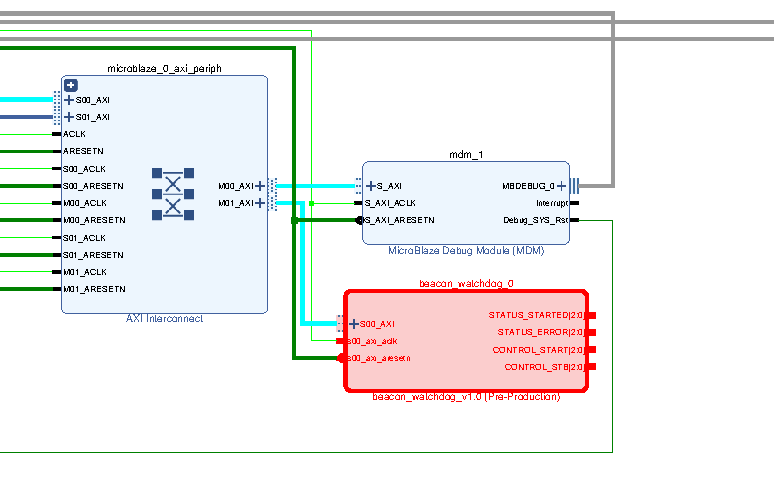
\includegraphics[width=0.9\linewidth]{images/chapter4/wd_ip_inst_cropped2.pdf}
\caption{Instantiation of the Watchdog IP.}
\label{fig:wd_ip_inst}
\end{figure}

As conceptually shown in Figure \ref{fig:rs2}, the IP presents two interfaces:
\begin{itemize}
    \item \textit{S00\_AXI}: The AXI interface is used to communicate with the watchdog from an AXI master. It includes the s00\_clk and s00\_rstn signals.
    \item \textit{Custom Interface}: The custom interface is meant to expose some signals towards other peripherals that may or may not need it. Each of those signals is a vector of 3 sub-signal, one for each watchdog module. In particular, the \textit{CONTROL\_START} and \textit{CONTROL\_STB} are directly connected to the register's bits Start and Kick without any TMR transformation. The \textit{STATUS\_STARTED} and \textit{STATUS\_ERROR} are instead the TMR version of the watchdog's started and timeout signals, respectively.
\end{itemize}

The IP can be easily customized via a custom IP wizard or via TCL commands. The following is the GUI wizard:

\begin{figure}[H]
\centering
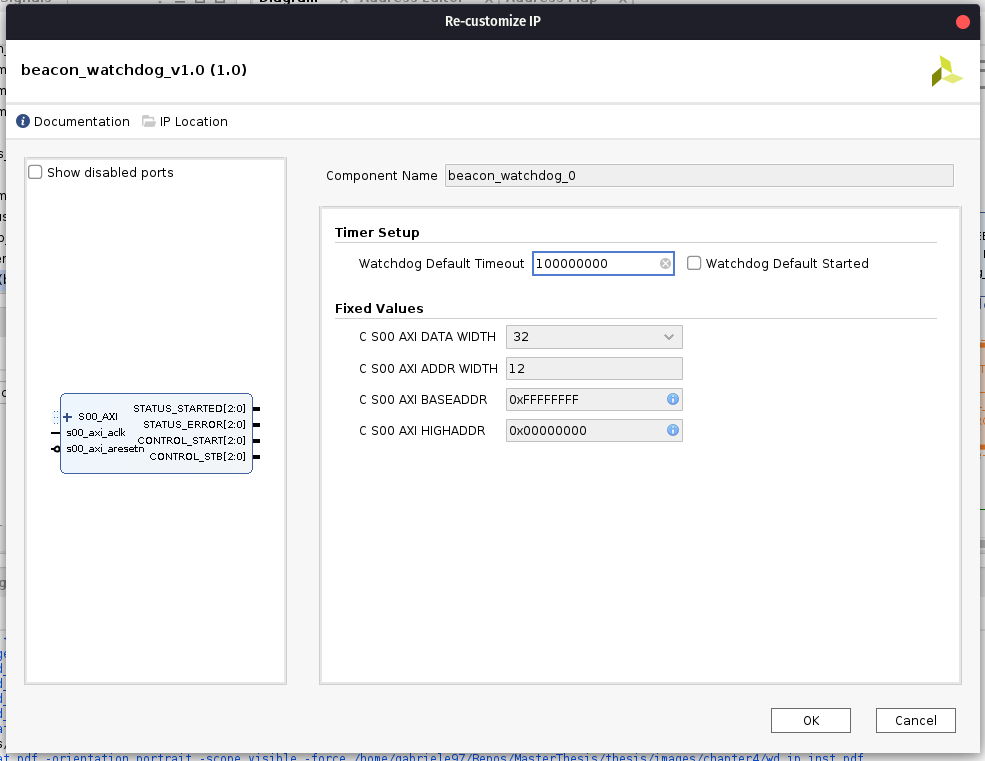
\includegraphics[width=0.8\linewidth]{images/chapter4/wizard_ip.png}
\caption{Watchdog IP configuration wizard.}
\label{fig:wd_ip_wizard}
\end{figure}

It is possible to set a custom initial value for the timeout register and the default start condition of the watchdog: if it is checked, at each reset the watchdog is immediately started without waiting for the \textit{Start} bit to be set. This can be useful for different purposes, but in particular for fault injection testing.\bigskip

Finally, when the IP is instantiated in a Block Design and the final .xsa file is generated, watchdog drivers are automatically inserted and ready to be used with Vitis. Thus, it is able to generate a Board Support Package (BSP) that contains and defines these new drivers.\bigskip

Follows an example of the usage of the drivers to control the watchdog. It demonstrates the usability of the final design, with a set of very high-level functions. The example demonstrates a possible way to organize the kicking act across the code to cover not only CPU hangs but also other faults (computational errors, self-test code, etc.).

\newpage
\begin{lstlisting}[style=C]
#include "beacon_watchdog.h"

/* header file for the hardware parameters, 
like peripheral addresses */
#include "xparameters.h" 
int main() {
  GBcnCtrl hBcn; //Handle to the watchdog
  uint32_t value;

  value = XPAR_BEACON_WATCHDOG_0_S00_AXI_BASEADDR;
  GBcnCtrl_Initialize(&hBcn, value);

  // Timeout set to 2 seconds (double of the watchdog's clk freq)
  GBcnCtrl_SetTimeoutValue(&hBcn, XPAR_CPU_CORE_CLOCK_FREQ_HZ<<1);
  GBcnCtrl_Start(&hBcn);

  value = hBcn.modules->module0.DATAREG;
  printf("Module 0 Timeout Value: %d\r\n", value);

  value = hBcn.modules->module1.DATAREG;
  printf("Module 1 Timeout Value: %d\r\n", value);

  value = hBcn.modules->module2.DATAREG;
  printf("Module 2 Timeout Value: %d\r\n", value);

  while(1) {
    checksum ^= (res += 2);

    // Example of self test check on checksum
    if(checksum & 0x3 == 0x0) {
      // FAULT!! Stop kicking, hardware needs to be reset!
      while(1); // Waiting for timeout expiration
    }

    // Kicking (automatic transition detection)
    GBcnCtrl_Toggle(&hBcn); 
  }

}
\end{lstlisting}

% add AXI testbench in appendix 

% IP, AXI interface, AXI registers and how they are connected to the FSM. How TMR is managed from the point of view of the registers.

\newpage
\section{Design with Partial Reconfiguration}

Partial reconfiguration is a way to change or update an FPGA design without the need to re-program the whole FPGA. Hence, it is possible to reprogram only a portion of the design without interrupting the rest of the design. In Xilinx's world, this is called \textit{Dynamic Function Exchange} (DFX).\bigskip 

There are different reasons why people do this. The main reason is \textit{area}: perhaps the FPGA is already full but more functions need to be pushed to the FPGA, and a way to achieve this is to partially reconfigure the design. Hence, the whole system is analyzed and blocks that are not used at the same time are grouped together. Each of the identified groups is assigned to a piece of FPGA fabric and that portion is marked as reconfigurable. 

\begin{figure}[H]
\centering
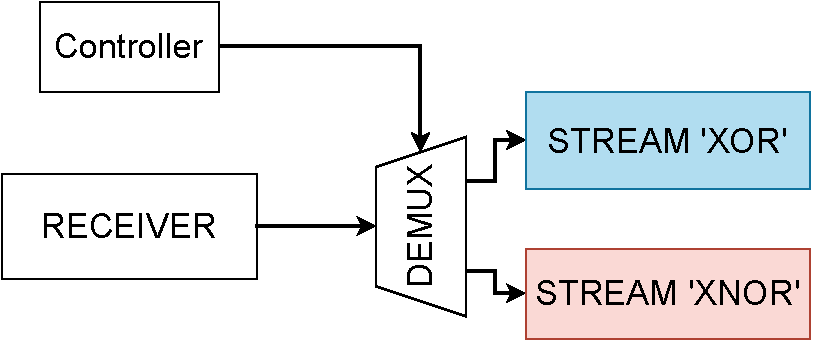
\includegraphics[width=0.8\linewidth]{images/chapter4/partial_modules.pdf}
\caption{Example of partial reconfiguration modules.}
\label{fig:partial_why}
\end{figure}

In the above figure, an example is shown. There is a receiver module that receives data from some source (it can be an Ethernet interface for instance). The system needs to compute a checksum of the received data, but not always in the same manner. Hence, two modules compute the checksum in two different ways. The whole design as it is does not fit in the FPGA, but luckily the two modules are not used at the same time so they can be grouped. The group is then marked as reconfigurable and the controller, before requesting to compute a checksum to the needed module, reconfigures the area with the module that the controller designed as the one needed to compute the checksum. In this way, the system continues to work in other sub-parts of the design, and meanwhile, the partial reconfiguration and the checksum computation are performed. The final design is the following:

\begin{figure}[H]
\centering
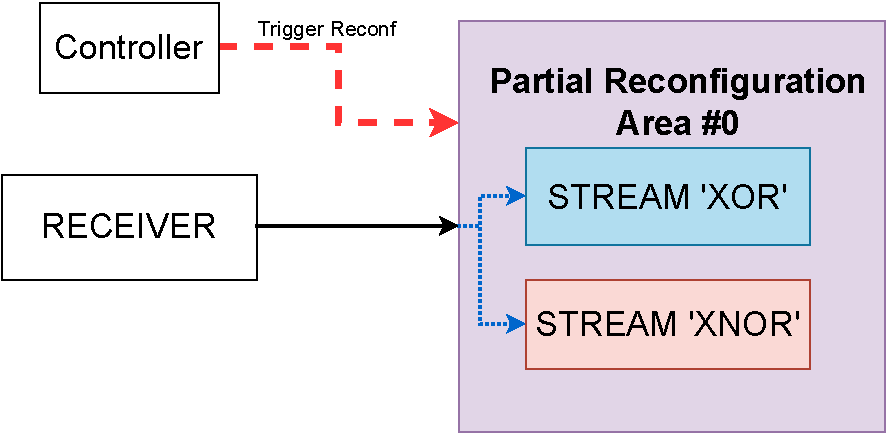
\includegraphics[width=0.8\linewidth]{images/chapter4/partial_modules_group.pdf}
\caption{Example of modules grouped under a partial reconfiguration area.}
\label{fig:partial_why_group}
\end{figure}

Furthermore, partial reconfiguration is not limited only to functionality exchange. It can be used to implement a \textit{partial scrubbing} of the design, for example when a fault affecting a reconfigurable area is detected. This is the case under study for what concerns this thesis work, as shown in Figure \ref{fig:reconf_scheme}. This allows to reconfigure the area without interrupting the rest of the design and mainly it is faster, reducing the down-time of the system, thus improving the overall availability. Moreover, the bit-flip causing the fault is definitely removed thanks to its reconfiguration.\bigskip

For what concerns Xilinx, the Dynamic Function Exchange is achieved by downloading a \textit{partial bitstream} into the FPGA via a \textit{Configuration Access Port} (CAP) that can be accessed directly from the FPGA itself. The partial bitstream is generated by adding some steps to the standard Vivado Design Flow. \bigskip

As explained in Section \ref{sec:raw_bitstream}, ZYNQ systems offer two dedicated ports, one for the PS and one for the PL. The PS port is the Processor Configuration Access Port (PCAP) and the PL port is the Internal Configuration Access Port (ICAP). As explained, they are mutually exclusive. 

% What is it. Tell about an example: module that can work in some way then it is reconfigured. Useful because maybe all the design doesn't fit in the FPGA but not all the design is needed at the same time so it can be reconfigured to change funcionality when needed. % take from video you followed, where at the beginning it explains how does it work.
% Then error fix.

\subsection{Vivado Design Flow for Dynamic Function Exchange}

Unluckily, Vivado versions prior to 2021.2 do not support DFX for Block Designs. Hence, for what concerns modules to be grouped under a partial reconfiguration partition, the designer must move the reconfigurable IP instances outside the Block Design and manually instantiate them in the top-level module. \bigskip

As a reference, a design with a custom 2-bit counter IP is used. The designer wants to have another counter IP to be used alternatively that is able to count up to 15 (4-bit counter), without using more area. Hence, the two counters are grouped under a partial reconfiguration partition. Each counter is defined as Reconfigurable Module (RM) and within a partition, only one RM at a time can be available. \bigskip

A reconfigurable partition is seen by other modules as the same component: other modules do not need to care about the reconfigurable module. Hence, a partition is defined by a single HDL wrapper with the same port definitions for all the modules in the partition. Thus, if there are two IPs and both of them have a CLK and Reset port and the third port is different (the first IP has a 2-bit port while the second one has a 4-bit port), a common definition needs to be found. In this simple case, the third port in the partition wrapper will have 4 bits and the IP with the 2-bit port is extended to four by fixing the higher bits at 0.\bigskip 

Through Vivado's IP Catalog, first, a \textit{Binary Counter} IP is instantiated with a 2-bit counter. Then a \textit{Binary Counter} IP is instantiated with a 4-bit counter. Once an IP is instantiated, a .xci file is generated. A .xci file is an XML file that records the values of project options, customization parameters, and port parameters used to create the IP. Once this is done, one wrapper for each IP must be created with the same port definition. The wrapper related to the 2-bit counter is instantiated in the top-level module. This means that the 2-bit counter is designed as the default module and it is inserted in the full bitstream, leading to a normal bitstream and design generated until now. Furthermore, there is a high chance that the reconfigurable modules (RMs) need something from the Block Design part. In that case, the designer must make available to the outside the needed signals to connect the reconfigurable modules, through the usages of Block Design's port definition both for input and output signals. \bigskip

% If the port definition among the two IPs differs in some way, the designer needs to define a new wrapper for the IP that differs. Inside the wrapper, the IP is instantiated and the additional glue logic is added. The hierarchy becomes:

% In the above example, \texttt{Counter_Wrapper} instantiatese the 2-bit counter by its own wrapper. This means that the 2-bit counter is designed as the default module that is inserted in the full bitstream. This means that during the first configuration, the 2-bit counter is loaded up by default.\bigskip

Once the sources are defined, the Vivado Project must be converted into a DFX-capable Project. This can be done via Tools $\rightarrow$ Enable Dynamic Function Exchange. This is an irreversible process. It is possible now to define a new partition with a right-click on the main wrapper and select \textit{Create Partition Definition}. Once the partition is created, it is possible to see it inside the \textit{Partition Definitions} tab. Here, a default reconfigurable module is created with the wrapper and the .xci file previously selected. It is possible to create a new reconfigurable module inside the partition where the .xci and wrapper of the second IP must be added (via a manual selection of the files).

\begin{figure}[H]
\centering
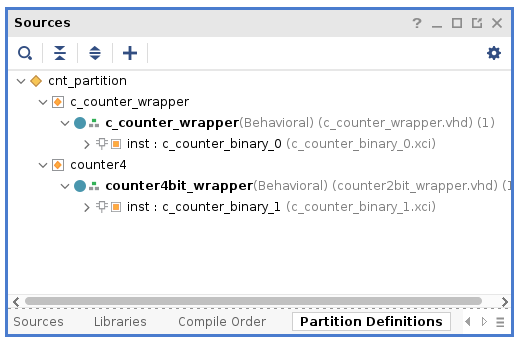
\includegraphics[width=0.80\linewidth]{images/chapter4/parts.png}
\caption{Partition definition with two reconfigurable modules, each one with its own wrapper and .xci file.}
\end{figure}

After the partition definition is completed, it is time to tell Vivado how the possible configurations for the various partitions are defined. Consequently, Vivado will be able to create bitstreams for each of the configurations indicated. To achieve this, on the left sidebar click on \textit{Dynamic Function Exchange Wizard}. For this simple example, there are two configurations: one with the 2-bit counter and the other with the 4-bit counter. \bigskip

Finally, it is possible to start the Synthesis process. After it has finished, a new set of contrainsts must be defined. In particular, the default wrapper instantiation (the one indicated in the top-level module) must be inserted in a PBLOCK. Once created, the PBLOCK is automatically set as \texttt{IS_SOFT = 0}. This represents the area of the FPGA marked as reconfigurable for the partition the instance belongs to.\bigskip

At this point, everything is defined and ready to be implemented onto the FPGA. If the Flow is executed until the final \textit{write_bitstream} step, the full bitstream is generated (as usual) and one partial bitstream for each of the configurations is generated. In particular, for each configuration a different run is executed, thus for each of them, the implementation and write_bitstreams steps must be performed. Of course, partial bitstreams have a lower size, where the size is logically direct proportional to the area of the PBLOCK:

\begin{table}[H]
\centering
\begin{tabular}{ l|lr }
    \textbf{Bitstream Type}&\textbf{Partition}&\textbf{Size}\\
    \hline
    Full&Whole Design&\texttt{3.9 MB}\\
    Partial&Count 2 Module&\texttt{640 KB}\\
    Partial&Count 4 Module&\texttt{640 KB}\\
\end{tabular}
\caption{Comparison between full bitstream and partial bitstreams sizes.}
\end{table}

As shown in the table above, the two partial bitstreams have the same size. This is because both of them reconfigure the same PBLOCK, thus the same area. It is possible to test the partial reconfiguration with XSCT using the following script, as an example:\bigskip

\begin{lstlisting}[style=tcl]
connect
target 4 # targets the FPGA

# loads the full bitstream
fpga design_1.bit 

# loads the partial bitstream after the full one has been loaded previously
fpga -partial design_1_inst_counter4bit_wrapper_partial.bit
\end{lstlisting}


% \begin{lstlisting}[style=tcl]

% # First IP: 2 bit
% create_ip -name c_counter_binary -vendor xilinx.com -library ip -version 12.0 -module_name c_counter_binary_0

% set_property -dict [list CONFIG.Output_Width {2}] [
%     get_ips c_counter_binary_0
% ]

% generate_target {instantiation_template} [
%     get_files /tmp/project_1/project_1.srcs/sources_1/ip/c_counter_binary_0/c_counter_binary_0.xci
% ]

% # Second IP: 4 bit
% create_ip -name c_counter_binary -vendor xilinx.com -library ip -version 12.0 -module_name c_counter_binary_1

% set_property -dict [list CONFIG.Output_Width {4}] [
%     get_ips c_counter_binary_1
% ]

% generate_target {instantiation_template} [
%     get_files /tmp/project_1/project_1.srcs/sources_1/ip/c_counter_binary_1/c_counter_binary_1.xci
% ]
% \end{lstlisting}

\subsection{DFX with MicroBlaze in Vivado 2021.1}

In the previous section, an example of Dynamic Function Exchange is presented. As explained, with versions of Vivado older than 2021.1, the DFX flow requires a manual instantiation and management of the various IPs involved in the reconfigurable part. With newer versions, indeed, a new feature called Block Design Containers (BDC) allows users to segment designs into multiple block designs, enabling modular and team-based design flows, including DFX flows. \bigskip

A BDC can be set as reconfigurable, turning it into a Reconfigurable Partition (RP) and enabling each design source within it to be considered an RM. The DFX Wizard populates each RP with all possible RMs for each RP before defining Configuration and Configuration Runs, similar to the RTL project flow for DFX. \bigskip

However, using simple IPs or simple HDL designs, the manual flow outside the Block Design tool is feasible. Unfortunately, when a designer wants to partial reconfigure a MicroBlaze, two problems arise, where the second one is a direct consequence of the first:

\begin{enumerate}
    \item deciding to partial reconfigure a MicroBlaze with the flow described previously becomes immediately unfeasible due to the high number of ports and signals to manually manage outside the Block Design environment. 
    \item softwares like Vitis are based on the description included in the .xsa file. This file is generated, as explained previously, using Vivado. This description file is exclusively based on the Block Design tool part of the project, because Vivado has no way to understand how the designer is connecting and configuring IPs outside the Block Design. Thus, working with Vitis becomes impossible because Vitis will tell the user that there is no MicroBlaze available in the design. 
\end{enumerate}

For what concerns this thesis work, a \textit{hack} is necessary to solve those problems. When the Block Design tool is used, internally Vivado creates a single HDL file (VHDL or Verilog, it depends on the settings of the project itself). This HDL file contains the whole description of the Block Design and all the necessary signal connections. This file can be copy-pasted in a completely different project and set as a top-level module. This is the chosen way to overcome the first problem: avoid manually instantiating the MicroBlaze IPs. This creates a new problem: all the IPs definitions (.xci files) used in the Block Design are not available in the new project, so it is not synthesizable basically. This problem can be easily solved by importing the IPs definitions from the original project to the new one. \bigskip

This new project is now ready to be configured and make the MicroBlaze a Reconfigurable Module inside its own reconfigurable partition. Hence, it is possible to follow the steps described in the previous section. The only operation to do \textit{manually} is to substitute the MicroBlaze instance with its own wrapper, that can be generated easily. Only a configuration is possible (in the most basic scenario as this one), thus Vivado generates only a partial bitstream together with the full bitstream as usual.\bigskip

The second problem is still there. From a purely HDL description of the design, Vivado is not able to generate a .xsa description. However, the two projects are practically the same, so the .xsa file originated from the base project can be extracted (it is essentially a .zip file) that contains a .xml description of the peripherals and memories, available CPUs, software drivers and the full bitstream to use to let Vitis program the FPGA. Basically, the bitstream can be substituted with the one generated by the second project (containing the Reconfigurable MicroBlaze) and the game is done.

\begin{figure}[H]
\centering
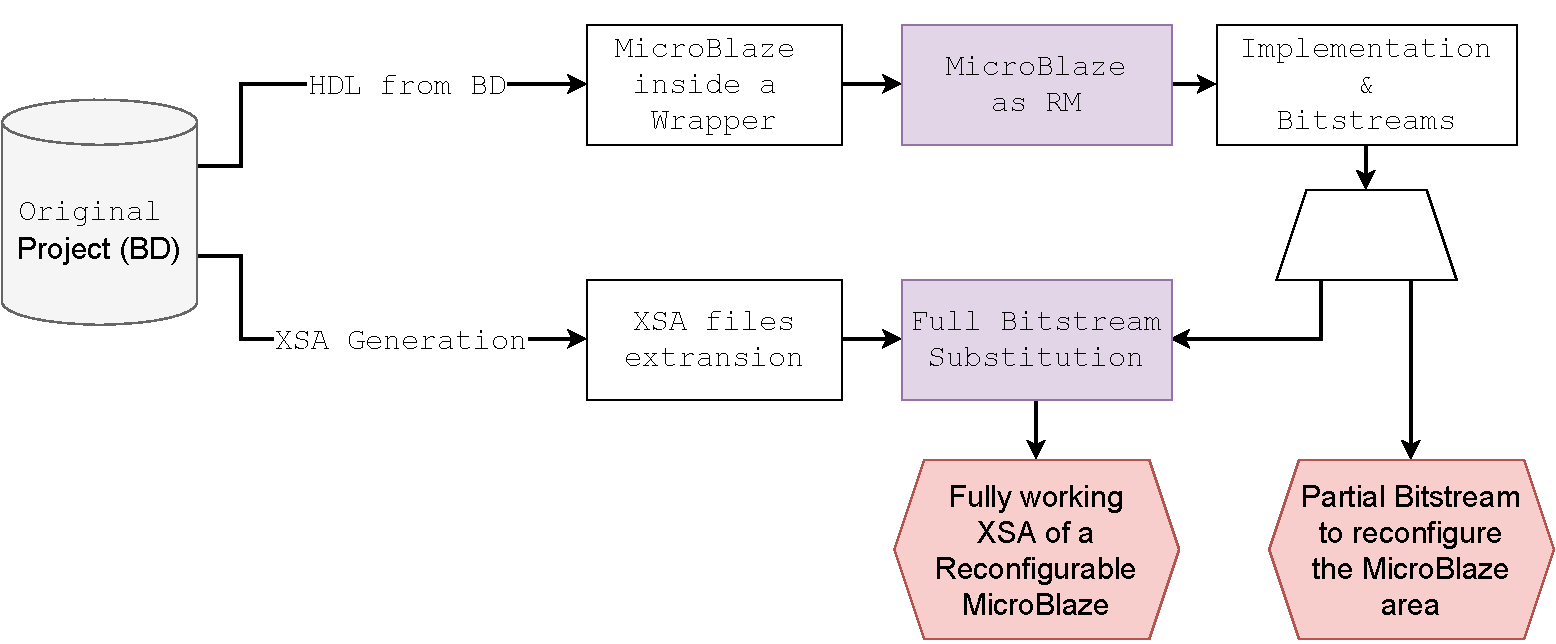
\includegraphics[width=1.0\linewidth]{images/chapter4/mystic_flow.pdf}
\caption{Flow used to generate a fully working Reconfigurable MicroBlaze design.}
\label{fig:mystic_flow}
\end{figure}

\subsection{Xilinx DFX Controller}
During the previous sections, DFX has been successfully achieved both for simple modules or for more complex one like a full MicroBlaze. However, there is still no way to perform the partial reconfiguration from within the FPGA itself. \bigskip

Luckily, Xilinx provides an IP that is able to manage the partial reconfigurations from within the FPGA and ease the process for designers and developers. It is the Xilinx Dynamic Function eXchange Controller (DFX Controller) IP core, that provides management functions for self-controlling partially reconfigurable designs. \bigskip

\begin{figure}[H]
\centering
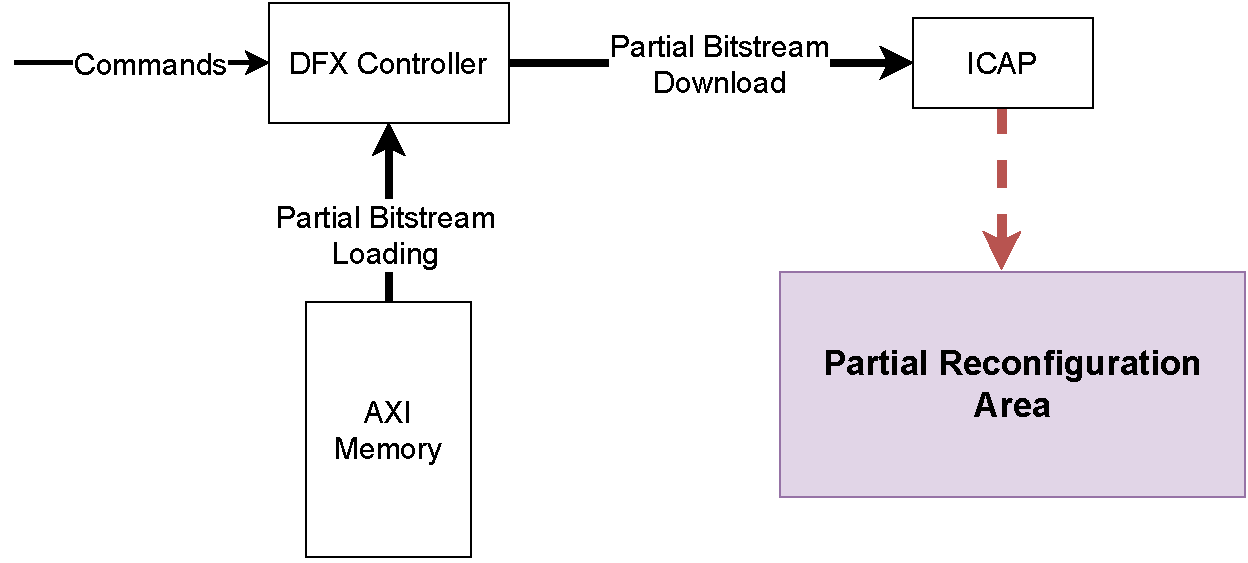
\includegraphics[width=0.9\linewidth]{images/chapter4/dfxc.pdf}
\caption{Basic scheme of the DFX Controller flow.}
\end{figure}

As shown in the figure above, the DFX Controller's main job is to fetch the partial bitstream data from an AXI memory peripheral and send it to the ICAP. This action is performed under certain commands (or triggers) sent from another actor in the system.\bigskip

The DFX Controller can be managed both statically via a GUI Wizard (or TCL) during the IP definition or dynamically from a CPU (like the MicroBlaze) or any other master in the system using a dedicated AXI interface. Internally it is organized as a series of Virtual Sockets. It supports up to 32 Virutal Sockets and each Virtual Socket can manage up to 128 Reconfigurable Modules. A Virtual Socket allows to manage all the RMs inside it as a group: it means that reset signals and other signals are shared between all the RMs inside it. \bigskip

For what concerns this thesis work, a Virtual Socket with a single Reconfigurable Module is enough to manage the MicroBlaze reconfiguration. For each Reconfigurable Module, the DFX Controller allows defining the memory address where the partial bitstream can be found and the size in bytes. Moreover, it allows to set up the type of reset required. In fact, when a module is reconfigured, it should be reset to be sure that it starts from a clean state. \bigskip

Last but not least, the DFX Controller allows to trigger a reconfiguration via:
\begin{itemize}
    \item a software trigger, via DFX Controller's AXI registers.
    \item a hardware trigger, via a dedicated interface.
\end{itemize}

\section{Integration of the watchdog and the DFX}
It is finally time to put everything together. The scheme to apply is shown if Figure \ref{fig:reconf_scheme}, where the watchdog is a simple IP that can be used to trigger the MicroBlaze reconfiguration when an error occurs. The DFX Controller is used to manage the reconfiguration process. 

\subsection{Partial bitstream storage}
The first problem to solve is the storage of the partial bitstream. As an example, the generated partial bitstream for the MicroBlaze RM measures 389928 bytes (around 380 KB). A possible storage solution would be the usage of the BRAMs available inside the FPGA and connecting them to the AXI bus via the AXI Interconnect using a Local Memory Controller IP. Unluckily, the used FPGA does not have so many BRAMs available (and a few are used as Instruction and Data memory for the MicroBlaze itself), thus this solution is unfeasible. The proposed solution is to use the on-board DDR memory, which offers 512 MB of storage easily accessible via the AXI bus by enabling the Slave interface \textit{S\_AXI\_HPO} in the PS's IP (ZYNQ7 Processing System IP). This interface can be connected to the AXI Interconnect as other slaves, like the peripherals. Once connected, all the masters in the AXI Bus can access the PS's internal address space from \texttt{0x00000000} to \texttt{0x1FFFFFFF}. As shown in Table \ref{tab:zynq_memory_map}, at address \texttt{0x00000000} there is the On-Chip Memory (OCM) where usually the ARM cores executes the code from. To avoid conflicts, only the second half of the DDR is used (so from \texttt{0x10000000} to \texttt{0x1FFFFFFF}). \bigskip

To make things easier, the partial bitstream is statically inserted in the .elf file executed by one of the two ARM cores. To achieve this, the partial bitstream is first converted to a C array of 32-bit items, via a script explained in Section \ref{sec:script_header}. However, this is not enough because the array would be allocated in the \texttt{.text} section of the .elf file, that is placed at low memory addresses (below the \texttt{0x10000000} target). To solve this, in the linker script generated by Vitis (regarding the ARM0 project), a new memory portion is defined: it points to the second half of the DDR memory. Then, a new section called \texttt{.partialbs} is created. The following is an extract of the linker script:\bigskip

\begin{lstlisting}[style=preformatted]
/* Define Memories in the system */
MEMORY
{
   ps7_ram_0 : ORIGIN = 0x0, LENGTH = 0x30000
   ps7_ram_1 : ORIGIN = 0xFFFF0000, LENGTH = 0xFE00
   /*2nd DDR half*/
   2ndhalf	 : ORIGIN = 0x10000000, LENGTH = 0x10000000 
}
/* Define the sections, and where they are mapped in memory */
SECTIONS
{
  .text : {
    KEEP (*(.vectors))
    *(.boot)
    *(.text)
    /*-------*/
    *(.vfp11_veneer)
    *(.ARM.extab)
    *(.gnu.linkonce.armextab.*)
  } > ps7_ddr_0
/** other sections **/
  .partialbs : {
    *(.partialbs)
  } > 2ndhalf
}
\end{lstlisting}

GCC (the C compiler used by Vitis) allows to map memory regions as preferred as well as to force the placement of a certain variable in a certain place in memory. This can be achieved as follows:

\begin{lstlisting}[style=C]
u32 __attribute__((section(".partialbs"))) data[] = {
  0xFFFFFFFF,
  0xFFFFFFFF,
  0xFFFFFFFF,
  0xFFFFFFFF,
  0xFFFFFFFF,
  0xFFFFFFFF,
  /**....**/
  0xAA995566, // SYNC WORD
  /**....**/
};
\end{lstlisting}

\subsection{How to enable the ICAP port}
For this work, the ARM core is not only used to load the partial bitstream in memory. As explained previously, the ARM cores hold full control of the two configuration ports (ICAP and PCAP) for security purposes. Before executing the partial configuration, the ARM core must release the hold on the ICAP and this is done in two consecutive steps:
\begin{enumerate}
    \item The ARM core disables the PCAP (because they are mutually exclusive).
    \item The ARM core enables the ICAP.
\end{enumerate}

This can be done easily with the XDevCfg driver offered by Xilinx:

\begin{lstlisting}[style=C]
#include "platform.h"
#include "data.h" // Contains the partial bitstream array
#include "xdevcfg.h"

int main() {
  XDcfg XDcfg_0;

  XDcfg_Config *conf = XDcfg_LookupConfig(XPAR_XDCFG_0_DEVICE_ID);
  XDcfg_CfgInitialize(&XDcfg_0, conf, conf->BaseAddr);
  XDcfg_DisablePCAP(&XDcfg_0);
  XDcfg_SelectIcapInterface(&XDcfg_0);

  while(1);
}

\end{lstlisting}

% Explain bitstream storage. DDR in this case, protected, blah blah. Linker script. Firmware to disable the PCAP in the ARM core.

\subsection{ICAP instantiation}
The second last step is to connect the DFX Controller to the ICAP port. For security reasons, it is not directly available to the user. It is an HDL primitive that needs to be manually instantiated in the design so it needs to be manually inserted in the HDL code generated by the Block Design Tool and connected to the ICAP interface of the DFX Controller. \bigskip

The ICAP port can be accessed via different blocks, but the most simple is the ICAPE2. It offers different input and outputs port, as shown below:

\begin{figure}[H]
\centering
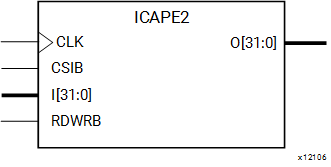
\includegraphics[width=0.4\linewidth]{images/chapter4/icap.png}
\caption{ICAP Interface.}
\end{figure}

The following is a short description of the ports:

\begin{table}[H]
\centering
\begin{tabular}{ c|r|p{8 cm} }
    \textbf{Port}&\textbf{Data Width}&\textbf{Description}\\
    \hline
    \texttt{CLK}&\texttt{1 bit}&The clock signal (max 100 MHz $\rightarrow$ 32 bit data bus $= 3.2 GB/s$).\\
    \texttt{CSIB}&\texttt{1 bit}&The chip select signal (active low).\\
    \texttt{RDWRB}&\texttt{1 bit}&The read/write signal.\\
    \texttt{I}&\texttt{32 bit}&The input data.\\
    \texttt{O}&\texttt{32 bit}&The output data.\\
\end{tabular}
\caption{ICAPE2 Interface description.}
\end{table}



% \begin{itemize}
%     \item \textit{CLK}: the clock signal (max 100 MHz $\rightarrow$ 32 bit data bus $= 3.2 GB/s$).
%     \item \textit{CSIB}: the chip select signal (active low).
%     \item \textit{RDWRB}: the read/write signal.
%     \item \textit{I[31:0]}: the input data.
%     \item \textit{O[31:0]}: the output data. 
% \end{itemize}

The ICAP interface can be use used to monitor (for example via a Integrated Logic Analyzer IP, as explained in Section \ref{sec:ila}) the configuration process when it is used as port for delivering bitstreams. The \texttt{O} port of the ICAPE2 block is a 32-bit bus, but only the lowest byte is used. The mapping of the lower byte is as follows:

\begin{center}
\begin{register}{H}{ICAP}{\texttt{O} port}% name=example
\regfieldb{}{24}{8}% READ_ONLY
\regfieldb{CFGERR\_B}{1}{7}%
\regfieldb{DALIGN}{1}{6}%
\regfieldb{RIP}{1}{5}%
\regfieldb{IN\_ABORT\_B}{1}{4}%
\regfieldb{}{4}{0}%
\begin{regdesc}\begin{reglist}[Request~Depth]
\item [CFGERR\_B]Configuration Error:\\0 = A configuration error has occurred.\\1 = No configuration error.
\item [DALIGN]Sync word (\texttt{0xAA995566}) received:\\0 = No sync word received.\\1 = Sync word received.
\item [RIP]Readback in Progress:\\0 = No readback in progress.\\1 = A readback is in progress.
\item [IN\_ABORT\_B]ABORT in progress.\\0 = Abort is in progress.\\1 = No abort in progress.
\end{reglist}\end{regdesc}
\end{register}
\end{center}

The following is the VHDL code for instantiating the ICAP port in a design:

\begin{lstlisting}[style=VHDL]
ICAPE2_inst : ICAPE2 generic map (
   DEVICE_ID => X"3651093",     -- Simulation only.
   ICAP_WIDTH => "X32",         -- Input/Output data width.
   SIM_CFG_FILE_NAME => "NONE"  -- Simulation only.
) port map (
   O => O,         -- 32-bit output: Configuration data output bus
   CLK => CLK,     -- 1-bit input: Clock Input
   CSIB => CSIB,   -- 1-bit input: Active-Low ICAP Enable
   I => I,         -- 32-bit input: Configuration data input bus
   RDWRB => RDWRB  -- 1-bit input: Read/Write Select input
);
\end{lstlisting}

An example of the ICAPE2 during the initial phases of the configuration process is shown in Figure \ref{fig:icap_ila}. When the trigger is asserted (\texttt{vsm\_VS\_0\_hw\_triggers\_1}), the DFX Controller starts sending the configuration data taken from the partial bitstream uploaded in the memory. The ICAP's \texttt{O} port initially is at \texttt{0x9B} that means \textit{no cfg error}, \textit{no sync word}, \textit{no readback in progress}, \textit{no abort in progress}. When the SYNC WORD is received, the ICAP's \texttt{O} port is updated to \texttt{0xDB}: only 1 bit changed, indicating that the sync word was received.

\begin{figure}[H]
\centering
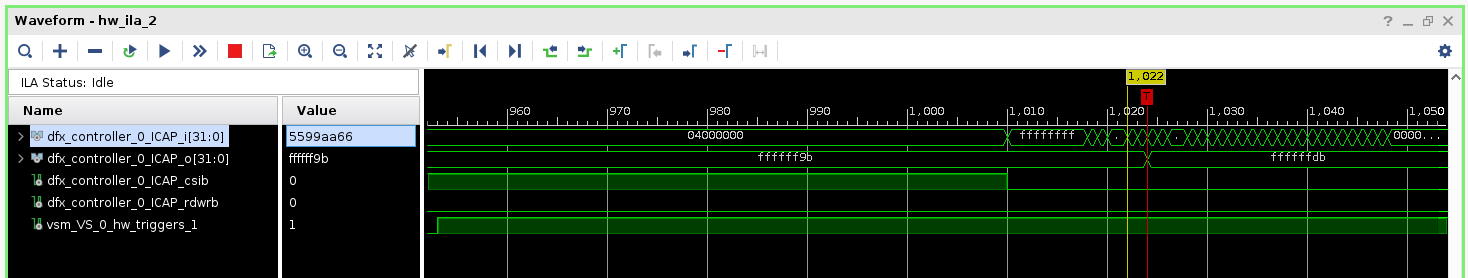
\includegraphics[width=0.95\linewidth]{images/chapter4/ila_icap.png}
\caption{ICAP Interface as seen by an ILA core.}
\label{fig:icap_ila}
\end{figure}

\subsection{Connection of the Watchdog and the DFX Controller}
All the actors are now ready to be integrated. In particular, the \textit{timeout} signal of the watchdog should be used as a trigger for the DLX to start the reconfiguration. Moreover, when the DFX finishes the reconfiguration, both the MicroBlaze and the Watchdog must be reset to avoid any unexpected behavior and to restart the watchdog's timer itself (as explained in Section \ref{sec:wd_impl}, the watchdog is designed to remains in the \textit{DOOMED} state until a reset arrives). \bigskip

First, the DFX Controller is configured to allow hardware triggers. This means setting up a signal width of 1 bit for the \texttt{vsm\_VS\_0\_hw\_triggers} signal and to assign the MicroBlaze RM previously configured as the RM to load when the triggers arrive. The problem is that the watchdog outputs a 3-bit wide signal as a timeout signal, due to the TMR design. This can be used to feed a final voter to convert a 3-bit wide signal to a 1-bit wide signal. At this point the voter represents a single point of failure, but as explained the probability of its failure is low. However, if its probability is not sufficiently low, it is possible to use a different voter implementation like the following one:

\begin{figure}[H]
\centering
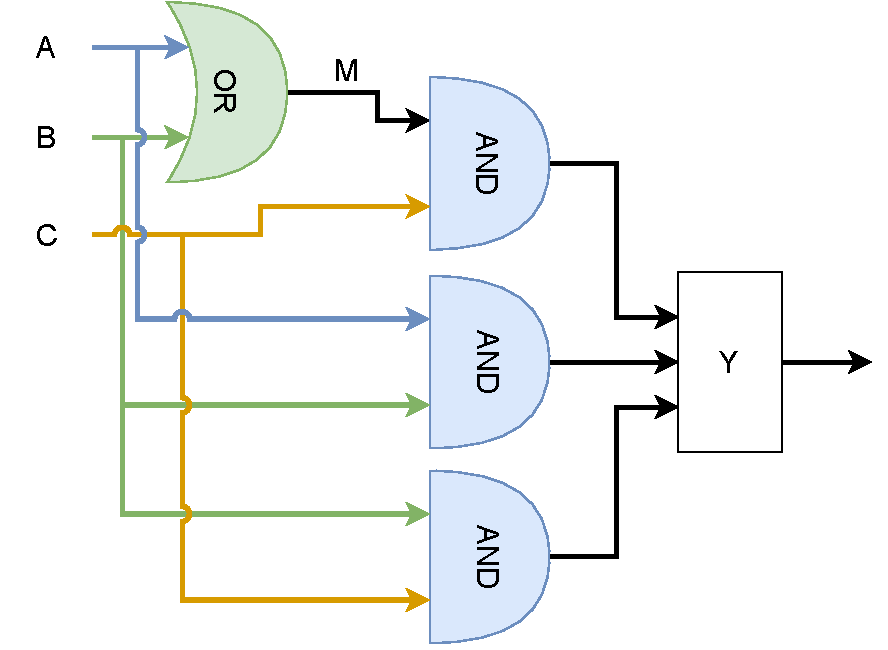
\includegraphics[width=0.40\linewidth]{images/chapter4/voter_enh.pdf}
\caption{Enhanced majority voter design.}
\end{figure}

The above scheme \cite{al} is made of a 1-bit OR gate, three 2-bit AND gates and a 3-bit OR gate. This design allows reaching a higher Fault Masking Ratio (FMR), specified as the ratio of the total number of correct voter output states in the presence of internal and/or external faults, which are masked, divided by the total number of potential internal and/or external fault occurrences. From the given definition, it may be understood that FMR has to be high (ideally 1) to achieve good (absolute) fault tolerance. A normal majority voter has an FMR of 42.86 \% while the enhanced majority voter has an FMR of 75.00 \%.\bigskip

Secondly, when the DFX Controller ends the reconfiguration process, the signal \texttt{vsm\_VS\_0\_rm\_reset} is asserted for 1 clock cycle, as specified in the RM's configuration. This is conncted to the \texttt{Reset} signal of the MicroBlaze that is active high, feeding an OR gate together with the active-high \texttt{mb\_reset} signal arriving from the \textit{Processor System Reset} IP. In this way, both the DFX Controller and the PSR are able to reset the CPU when required. \bigskip

To reset the watcdog, the reset signal needs to be negated because the Watchdog's reset signal is active low, as other AXI IPs are. Because the Watchdog can be reset both by the DFX Controller and the PSR, as for the MicroBlaze, a NOR gate is fed with the one coming from the DFX Controller and the one coming from the PSR in the active-high form, that is \texttt{peripheral\_reset}.\bigskip

Finally, the DFX Controller's ICAP port is connected to the ICAPE2's instance. The DFX Controller ICAP's \texttt{I} port is connected to the ICAPE2's \texttt{O} port, and the DFX Controller ICAP's \texttt{O} port is connected to the ICAPE2's \texttt{I} port.

% connection of the DFX to the watchdog and to the ICAP. Reset logic from the DFX controller to the ublaze and to the watchdog

% DFX connected to the watchdog via the hw trigger. How? Final voter.
% ICAPE2. DFX Decoupler.

\subsection{DFX Decoupler: what is it?}
There is one important aspect that was not mentioned in the previous sections. During the Partial Reconfiguration of a partition, unpredictable signal activity can happen between the Reconfigurable Partition and the remaining part of the system. To overcome this problem, Xilinx provides the Dynamic Function eXchange (DFX) Decoupler IP, for a complete logical isolation capability for DFX designs. \bigskip

During the reconfiguration process, the DFX Controller asserts a decouple signal that remains high for the entire duration of the process. This signal is used to decouple the system from the logic under reconfiguration and avoid strange signal activities. For example, can happen that an AXI write request signal is asserted wrongly, leading to a modification of a random memory location with an unexpected value. By decoupling the AXI interface from the rest of the system, this can be avoided. 

\begin{figure}[H]
\centering
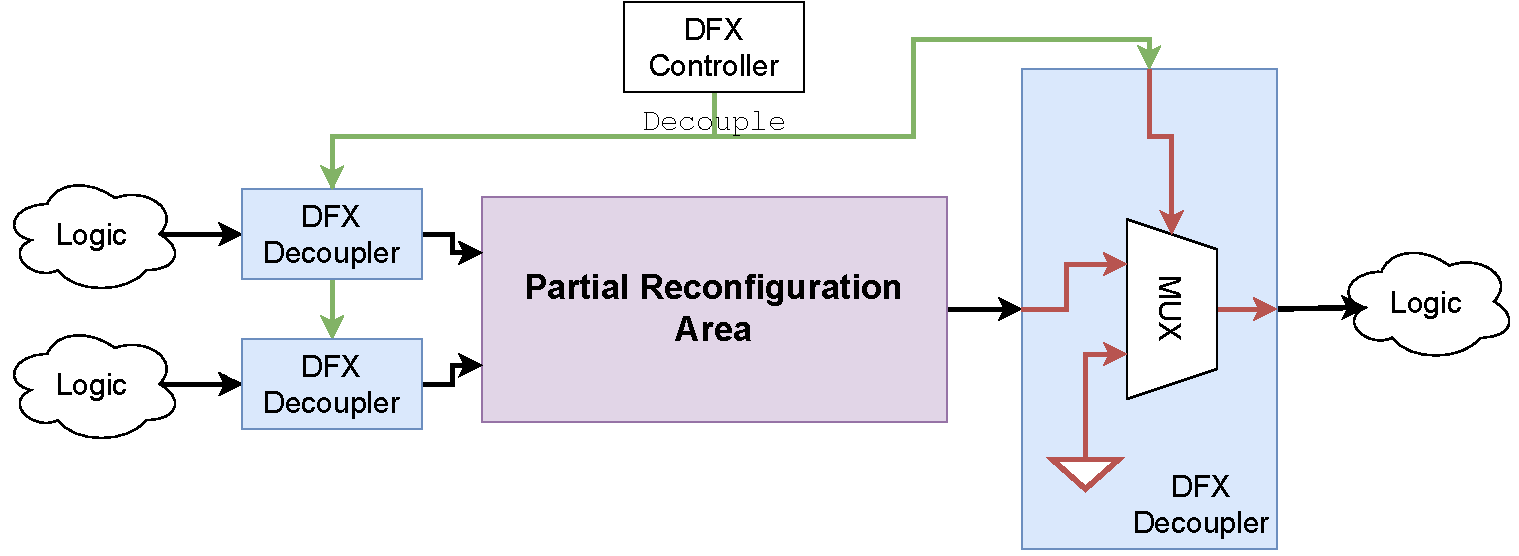
\includegraphics[width=0.95\linewidth]{images/chapter4/dfx_dec.pdf}
\caption{DFX Decoupler scheme.}
\end{figure}

In a complex system, like the case under study, there are a lot of signals that need to be decoupled. Luckily, the DFX Decoupler IP's Configuration Wizard offers the ability to create decoupler interfaces for each standard interconnection like AXI or LMB. For what concerns a simple MicroBlaze architecture, the following is the adopted solution:

\begin{figure}[H]
\centering
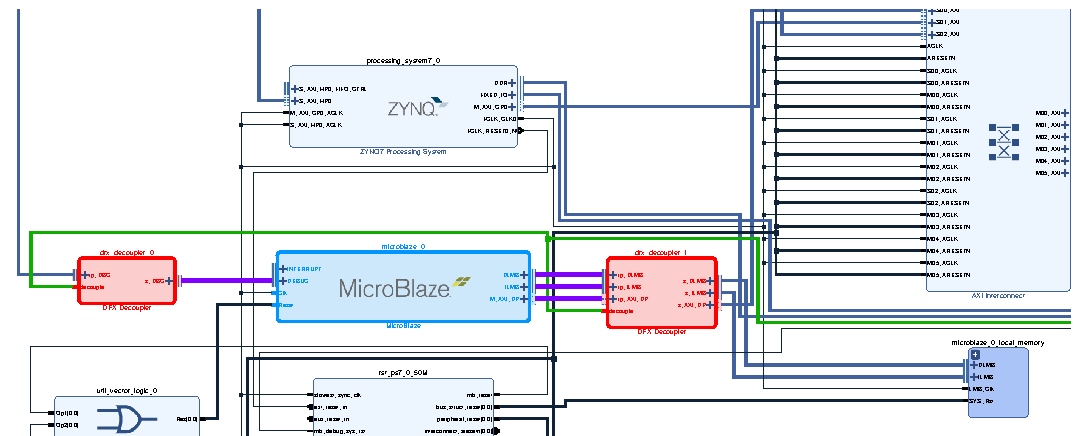
\includegraphics[width=0.95\linewidth]{images/chapter4/dec_mb-cropped.pdf}
\caption{Decoupling of a Reconfigurable MicroBlaze region.}
\end{figure}

\section{From a manual workflow to a fully automated one}

The presented workflow allows enabling partial reconfiguration of a MicroBlaze, even on an old version of Vivado. The workflow is presented in Figure \ref{fig:mystic_flow} and is made of 5 major steps, summarized as follows:

\begin{enumerate}
    \item Starting from a working project based on Block Design, with a MicroBlaze core, a DFX Controller and a Watchdog, the HDL description from the BD is extracted.
    \item A new project is created and the previous HDL description is copied into it. The MicroBlaze instance is replaced with its own wrapper and the wrapper instantiates the MicroBlaze. All the .xci files from the base project are copied into the new project.
    \item The new project is converted into a DFX-based project and the MicroBlaze wrapper is added in a new reconfigurable partition as Reconfigurable Module (RM). Finally, a PBLOCK is defined for the MicroBlaze wrapper.
    \item The new project is implemented and bitstreams are generated.
    \item From the base project, the XSA is generated, files within it are extracted and the bitstream is substituted with the one generated in the previous step. Then, all the files are inserted in a new .xsa archive to generate the new .xsa.
\end{enumerate}

Thus, the workflow is made of five simple steps that require a certain amount of time to be completed. The designer needs to execute all of them every time she/he wants to change something in the original project. Hence, the workflow is not suitable for a continuous integration process and some sort of automation is required. \bigskip

\subsection{The automatation script}

Luckily, all the flow can be almost easily scripted. In the following, the developed script is presented by dividing it into different subparts and each subpart is described by a dedicated pseudo-code algorithm. The overall flow is divided into five main blocks:

\begin{figure}[H]
\centering
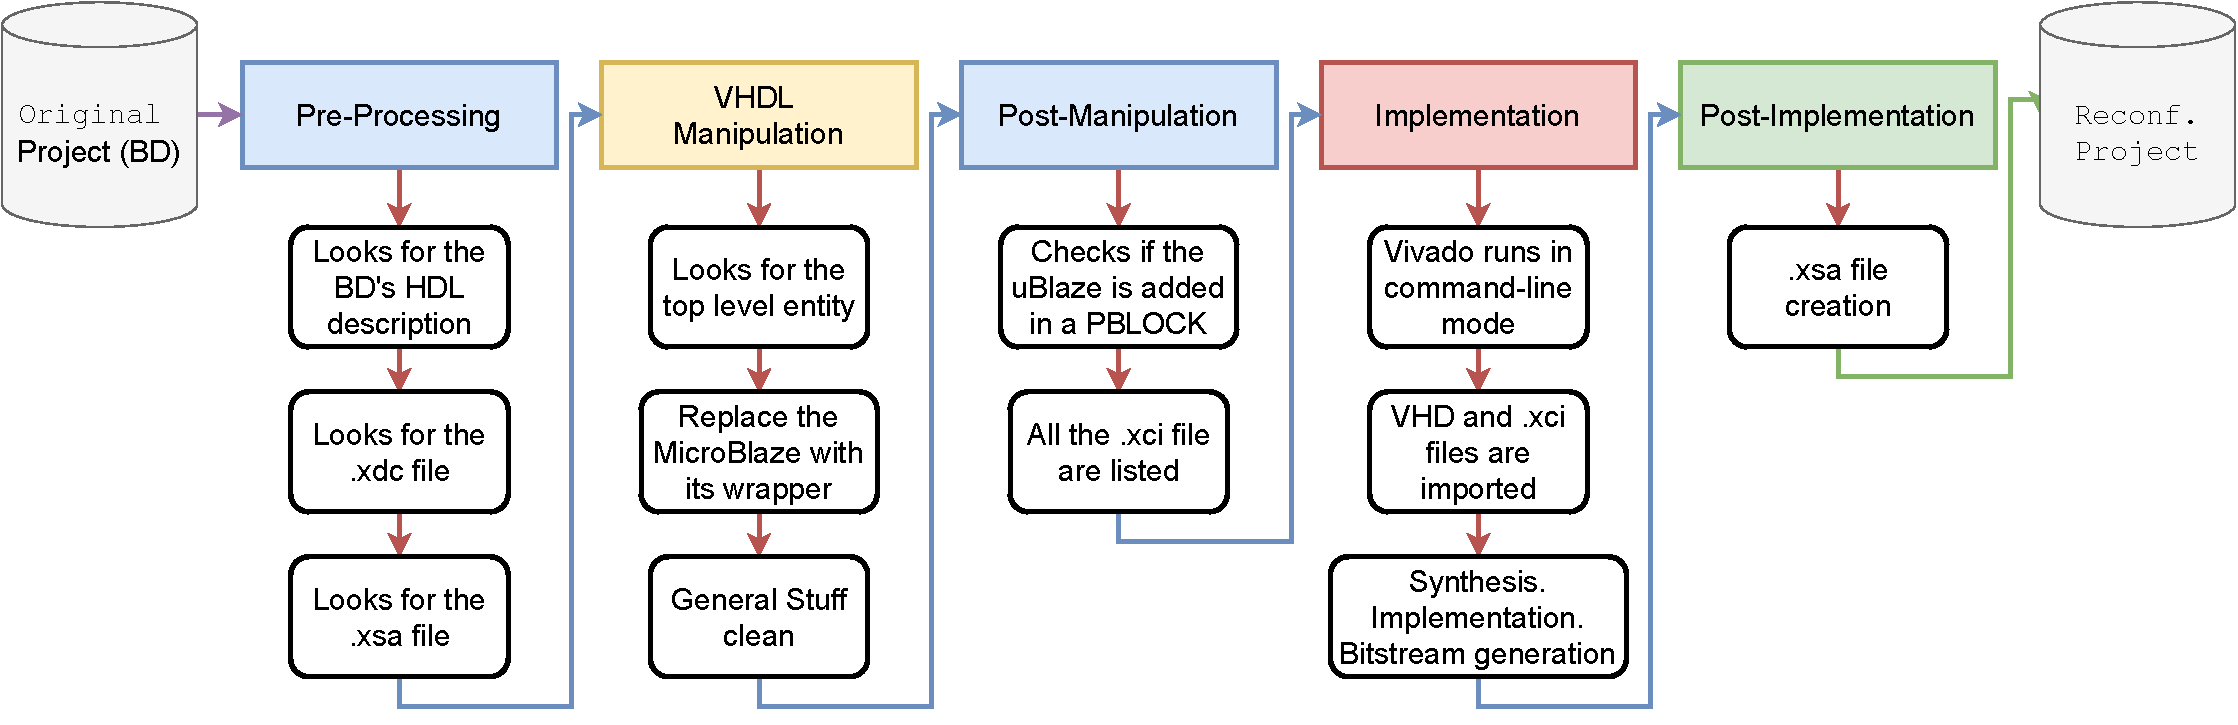
\includegraphics[width=0.95\linewidth]{images/chapter4/script_flow2.pdf}
\caption{Scheme of the script flow.}
\end{figure}

\subsubsection{Pre-processing block}
The pre-processing block is the first block to be executed in the automatic workflow script. It takes as input the original project path and checks if the project is a valid candidate for the workflow:

\begin{enumerate}
    \item Given the project path, the project name \texttt{\$pn} is extracted.
    \item The script checks for the existence of the \texttt{\$pn.gen} folder. This is a required folder that contains the generated HDL description of the Block Design. The script recursively checks for a path matching \texttt{*/bd/*/synth/\$dn.vhd}. If the path is found, means that the script knows the block design name \texttt{\$dn} and found its VHDL description file.
    \item The script searches any .xdc file that may contains the PBLOCK definition in the \texttt{\$pn.srcs} folder. However, the designer can supply its own .xdc file. The PBLOCK is not checked at this time.
    \item The script searches for the .xsa file. If not found, the script terminates asking the user to create it from within Vivado before running the script.
\end{enumerate}

\subsubsection{VHDL Manipulation block}
If the Pre-processing block runs successfully, the HDL Manipulation block can be executed. This is the most compilcated one. It takes as input the previous VHDL description file \texttt{\$dn.vhd} and a secondary VHDL file named \texttt{adding.vhd} that contains partial definitions of some hardware that the designer wants to add to the system outside the Block Design, like for example the ICAPE2. 

\begin{enumerate}
    \item The whole \texttt{\$dn.vhd} file is parsed. Each entity is extracted and stored separately in a list of entities. Each entity is made of libraries, entity definition and architecture content. The same is done for the \texttt{adding.vhd} file.
    \item Each entity is analyzed, looking for a MicroBlaze instance in its architecture. If found, the entity is marked as the top-level entity. The user can decide to indicate another entity as top level one, if the found entity is not the one he wants to use or if it is wrong. Each of the next steps is performed on the top-level entity.
    \item The script looks for the MicroBlaze's component declaration. 
    \item The script looks for the MicroBlaze instance, given the previous component name.
    \item The script creates a new entity, named \texttt{ublaze\_wrapper} and:
        \begin{enumerate}
        \item Extracts the ports declaration from the MicroBlaze component and adds them to the new entity ports definition. The entity part of the whole wrapper is created.
        \item The architecture is defined. First, the original MicroBlaze component is appended as it is, then it is instantiated and each port is connected to the ports of the entity wrapper under creation.
        \item The newly created entity is saved in a new file \texttt{ublaze\_wrapper.vhd}.
        \end{enumerate}
    \item The original microblaze component is replaced by the new wrapper component. The instance is left as it is, only the instance name is changed, referencing the new wrapper component.
    \item Some synthesizer attributes referenced to the older MicroBlaze instance are now referenced to the new wrapper instance.
    \item If in the base project, the DLX Controller's ICAP interface is made external through a port, Vivado automatically creates some attributes and entity ports to let them connect outside. They are removed.
    \item The definitions from the \texttt{adding.vhd} file are now merged. For each component in the architecture defined in the \texttt{adding.vhd} file, the script adds both the component and the relative instance to the top entity. It looks for the ICAPE2 instance too and adds it to the top entity (it is trated as special, becuase in this case there is no component declaration as other components).
    \item All the entities are appended in a new file \texttt{top.vhd}.
\end{enumerate}

\subsubsection{Post-manipulation block}
This is the third last block to be executed. At this point in time, if everything succeeded, the script knows the top-level name, the MicroBlaze instance name and any other useful information about the design. It proceeds with the following steps:

\begin{enumerate}
    \item The script knows the MicroBlaze wrapper instance name and now looks for the PBLOCK where it is assigned in the previous found .xdc file. If this is not found, the script terminates with an error.
    \item The script prepares a list of all the .xci files in the base project. It searches for possible .xci file related to the \texttt{adding.vhd} file in the \texttt{adding_xci} folder and appends them too.
\end{enumerate}

\subsubsection{Implementation block}
Now the scripts created all the files and information to create a new project and implement it. Vivado is launched in command-line mode and a TCL script is sourced to perform the following steps:

\begin{enumerate}
    \item The script creates a new project and VHDL is set as the active language.
    \item Imports the \texttt{top.vhd}, \texttt{ublaze\_wrapper.vhd} and the .xdc file into the new project.
    \item Takes the .xci list previously prepared and adds each file to the new project. They are references to the original files, not a copy.
    \item Enables the project as a DFX-based project. Creates a definition partition and a reconfigurable module. The wrapper is added to the partition. A single reconfigurable configuration is created.
    \item The project is synthesized and implemented. The bitstreams are generated both in .bit and .bin formats.
\end{enumerate}

\subsubsection{Post-implementation block}
This is the last block to be executed. It takes as input the generated full bitstream and the previously found .xsa file. The scripts unzip the .xsa file, substitute the old bitstream with the new one and re-zip the .xsa file.


\subsection{Script for partial bitstream to C header generation}
\label{sec:script_header}

Because of the choice to store the partial bitstream in memory by using the same .elf file executed by the ARM core to configure the PS, a script is needed to generate the C header file that contains the partial bitstream. \bigskip

An error to avoid is the usage of the bitstream in the .bit format instead of the .bin one to perform a partial reconfiguration via the ICAP interface. As explained in Section \ref{sec:bitstream_struct}, the difference between the two is that the .bit format contains a header while the .bin format does not. Hence, the header can have a different length, depending for example on the design name chosen by the user, thus can create an offset inside the bitstream. As an example, it can shift the SYNC WORD by 8 bits. The ICAP interface is not able to evaluate the header nor is capable of evaluating a shifted bitstream. Hence, the ICAP remains in the \textit{NOSYNC} state or it goes in the \textit{CFGERR} state. The .bit file is only useful to Vivado and XSCT because of the header, otherwise, it is only a waste of memory and must be not used outside Vivado tools.\bigskip

The script's job is to prepare a \texttt{u32} C array and fill it with the content of the partial .bin bitstream. The script allows the creation of an array with a specific size. It accomplishes this by adding some \texttt{NOP} instructions to the array at the end, only if the size of the bitstream is less than the required one. This can be useful if the DFX Controller is configured with a specific size for the partial bitstream to be loaded, and the designer discovers only at the end that the generated partial bitstream is smaller than the configured one. In this way, is possible to avoid changing the DFX Controller's settings and to perform the implementation again. \bigskip

Moreover, the script allows writing the content in little-endian or big-endian format. This is useful because if the bitstream is saved in memory with the wrong format and the ICAP reads it, it does not recognize the SYNC WORD and hence does not performs the partial reconfiguration.\bigskip

The following is an example of the script's usage:
\begin{lstlisting}[style=preformatted]
format=big
required_size=389928
align=0 # do not touch!
output=data.h

./to_header path/to/partial.bin $format $required_size $align > $output
\end{lstlisting}

